\documentclass[10pt]{article}
\usepackage[margin=0.75in]{geometry}
\usepackage{amsmath, amsthm, amssymb}
\usepackage{mathtools}
\usepackage{hyperref}
\usepackage{url}
\usepackage{subfiles}
\usepackage{enumitem}
\usepackage{setspace}
\usepackage{scalefnt}

\numberwithin{equation}{section}

%\usepackage{titlesec}

\usepackage{algorithm}
\PassOptionsToPackage{noend}{algpseudocode}
\usepackage{algpseudocode}
\RequirePackage{fix-cm}

\usepackage{nicematrix}

\usepackage{mdframed}
\mdfdefinestyle{bframe}{%
    outerlinewidth=1pt,
    innertopmargin=0,
    innerbottommargin=5pt,
    innerrightmargin=8pt,
    innerleftmargin=8pt,
    backgroundcolor=white
   }
   
  
\usepackage{chngcntr}

\counterwithin*{equation}{section}
\usepackage{scalerel}
%\newcommand\plus{\scaleobj{0.5}{+}}

% \titleformat{<command>}[<shape>]{<format>}{<label>}{<sep>}{<before-code>}[<after-code>]
\usepackage[small]{titlesec}
%\titlelabel{\thetitle.\;}
%\titleformat{\subsection}[runin]{\normalfont\bfseries}{}{1pt}{}[:]

%\titleformat*{\section}{\large\bfseries}
%\titleformat*{\subsection}{\normal\bfseries}
%\titleformat*{\subsubsection}{}
%\titleformat*{\paragraph}{\large\bfseries}
%\titleformat*{\subparagraph}{\large\bfseries}


\newcommand{\+}{%
	\raisebox{0.18ex}{\scaleobj{0.55}{+}}
%  \raisebox{\dimexpr(\fontcharht\font`X-\height+\depth)/2\relax}{\scaleobj{0.5}{+}}%
}

\DeclareMathOperator*{\argmax}{arg\,max}
\DeclareMathOperator*{\argmin}{arg\,min}

\DeclareMathSymbol{\shortminus}{\mathbin}{AMSa}{"39}

\usepackage{dsfont}

\newtheorem{proposition}{Proposition}
\newtheorem{definition}{Definition}
\newtheorem{corollary}{Corollary}
\newtheorem{remark}{Remark}
\newtheorem{lemma}{Lemma}

\theoremstyle{definition}
\newtheorem{example}{Example}[section]

\newcommand{\inv}{^{\raisebox{.2ex}{$\scriptscriptstyle-1$}}}
\newcommand\sbullet[1][.5]{\mathbin{\vcenter{\hbox{\scalebox{#1}{$\bullet$}}}}}
\newcommand\numberthis{\addtocounter{equation}{1}\tag{\theequation}}
\newcommand{\bigzero}{\mbox{\normalfont\Large\bfseries 0}}
\newcommand{\rvline}{\hspace*{-\arraycolsep}\vline\hspace*{-\arraycolsep}}


\title{\vspace{-2.0em} \vspace{-0.5em}}
\author{Matt Piekenbrock}
\date{}

\begin{document}
\noindent



\section{Introduction}
\subsection*{Motivation} TODO 
%\subfile{intro_feature}
%\subfile{overview} % Contributions, Main result overview, etc. 
\\
\noindent 
\textbf{Contributions: }
In this effort, we introduce an iterative $\epsilon$-approximation method for computing the \emph{the persistent counting invariants}---$\mu_p^{\ast}$ and $\beta_p^\ast$---in \emph{essentially} $O(m)$ memory and $O(mn)$ time, where $m, n$ are the number of $p+1, p$ simplices in the complex, respectively. 
The approximation method is spectral-based and is particularly efficient when frequent recomputation is needed on perturbed inputs, which we generically refer to as the \emph{parameterized setting}. 
We show that, when the accuracy parameter $\epsilon$ is made small enough, both invariants are recovered exactly. 
In deriving the approximation, we naturally obtain continuous variations of the counting invariants which are smooth and differentiable on the positive semi-definite cone, which we believe to be of independent interest. 
One particular advantage of the method is that, unlike other dynamic or ``kinematic'' computations, it does not require the complex $K$ be explicitly filtered nor does it require any complicated data structure maintenance procedures.
Indeed, as algorithm does not modify the boundary matrix $\partial(K)$ at all, it need not necessarily have $\partial(K)$ stored in memory at all.
%We find the approximation to also be efficient in practice: the complexity reduction does not use Zigzag persistent homology~\cite{milosavljevic2011zigzag} nor does it rely on Strassen-like reductions to the matrix multiplication time $O(n^\omega)$.
Interestingly, our results also imply the existence of an subcubic, output-sensitive algorithm for computing persistence diagrams (via~\cite{chen2011output}) that inherits all of the aforementioned benefits and requires as its only input an boundary matrix-vector operator $x \mapsto \partial x$. 

\subsection{Organization}
Section~\ref{sec:background_notation} introduces the notation and background theory on which the rest of the paper depends. Included are some theoretical motivations for this work in subsection~\ref{sec:duality_pbn_dgm}, an illuminating derivation of the PBN in~\ref{sec:duality_pbn_dgm}, a time-varying parameterization of boundary matrix, and a brief recount of related work in persistence-related algorithms.
Section~\ref{sec:sec:methodology} contains the main results: the spectral relaxation of the counting invariants, the complexities of computing them, and their basic properties.
  

%In section~\ref{sec:betti_derivation}, we show how the PBN may be expressed as a sum of rank computations on unfactored boundary (sub)matrices. 
%By representing the boundary operators implicitly and exploiting a variety of properties of the rank function, we demonstrate the rank-based PBN expression admits certain computational advantages in both static and parameterized settings. 
%We show the $p$-th PBN of a filtered simplicial complex $K_\bullet$ may be computed in essentially quadratic time and linear storage, as opposed to the cubic time and quadratic storage complexity required by persistence.
Finally, we illustrate both the computational and practical advantages our expression has with a few applications in section~\ref{sec:applications}. 
%By exploiting a connection between the rank function and the spectrum of linear operators, we also introduce a spectral-based approach $(1-\epsilon)$-approximates the PBN. 

%We show that taking relaxation is permutation invariant, obeys certain inclusion-exclusion principles, and admits a notion of stability---all properties useful in parameterized settings. 
%We illustrate a few applications of the relaxation in section. 
%Moreover, we show our relaxation is \emph{interpetretable} as it satisfies certain basic ``Betti-like'' properties and we illicit its connections back to spectral graph theory. 

% ---- Background & Notation ---- 
\section{Background \& Notation}\label{sec:background_notation}
\subfile{background}

\subsubsection*{The duality between PBNs and Diagrams}\label{sec:duality_pbn_dgm}

% --- Counting measure multiplicity interpretation --- 
\subfile{counting_measure}

\subsection{Motivating Derivation}\label{sec:betti_derivation}
%In what follows, we briefly outline the computation of the 

% For the moment, we omit the subscript $t \in \mathrm{T}$ and focus on a fixed instance of time. 
Let $B_p(K_\bullet) \subseteq Z_p(K_\bullet) \subseteq C_p(K_\bullet)$ denote the $p$-th boundary, cycle, and chain groups of a given filtration $K_\bullet$, respectively. 
Additionally, let $\partial_p : C_p( K_{\bullet}) \to C_p(K_{\bullet})$ denote the boundary operator sending $p$-chains to their respective boundaries. 
With a slight abuse of notation, we also use $\partial_p$ to also denote the filtration boundary matrix with respect to an ordered basis $(\sigma_i)_{1 \leq i \leq m_p}$.
The $p$-th persistent Betti number $\beta_p^{i,j}$ at index $(i,j) \in \Delta_+^m$, where $\Delta_+^m  := \{ \, (i,j) \in [m] \times [m] : i < j \, \}$, is defined as: 
\begin{align*} \label{eq:pbn}
	\centering
	\beta_p^{i,j} = \mathrm{dim}(H_p^{i,j}) &= \mathrm{dim} \left ( Z_p(K_i) / B_p(K_j) \right ) \\
	& = \mathrm{dim} \left( Z_p(K_i) / (Z_p(K_i) \cap B_p(K_j) \right) \\
	& \numberthis = \mathrm{dim} \left( Z_p(K_i) \right) - \mathrm{dim}\left( Z_p(K_i) \cap B_p(K_j) \right ) 
\end{align*}
%The dimension of the boundary group $B_{p-1}(K_i)$ may be directly inferred from the rank of $\partial_p^{i}$, and the dimension of $C_p(K_i)$ is simply the number of $p$-simplices with filtration values $f(\sigma) \leq i$. 
While $\mathrm{dim}(Z_p(K_i)) = \mathrm{nullity}(\partial_p(K_i))$ and thus reduces to a rank computation, the intersection term---the persistence part---is more subtle. Zomorodian et al.~\cite{zomorodian2004computing} outline an algorithm to compute a basis for $Z_p(K_i) \cap B_p(K_j)$ via a sequence of boundary matrix reductions; their subsequent Theorem 5.1 reduces the complexity of computing PH groups with coefficients in any PID to that of computing homology groups. 
However, the standard homology computations require $O(m^2)$ space and $O(m^3)$ time to compute, implying either of these approaches to computing the PBN computation exhibits same complexity as the full persistence computation.

% Golub and Van Loan 

%Alternatively, both iterative and explicit projector-based methods~\cite{ben2015projectors} may also for the intersection term in~\eqref{eq:pbn}, though these projectors may still be expensive to compute. 
% TODO: elaborate more, give von neumann inequality 

In what follows, we outline a different approach to computing~\eqref{eq:pbn} that we argue is not only simpler and computationally attractive, but also amenable to acceleration in dynamic settings. 
To illustrate our approach, we require more notation. If $A$ is a $m \times n$ matrix, let $A^{i, j}$ denote the lower-left submatrix defined by the first $j$ columns and the last $m - i + 1$ rows (rows $i$ through $m$, inclusive). 
%Given an $n \times m$ matrix $A$, let $A[I, J]$ refer to the submatrix formed by taking rows in the set $I$ and taking columns in the set $J \subseteq [m]$. Let $L_{, j}$
%\begin{equation}
%	\begin{bNiceMatrix}[first-row,first-col]
%       & i        & j \\
%i      & A & A_{ii}  \\
%m\text{ - }i & A_{\overline{i}i} & A_{jj}
%\end{bNiceMatrix}
%\end{equation}
\begin{figure}
\centering
%	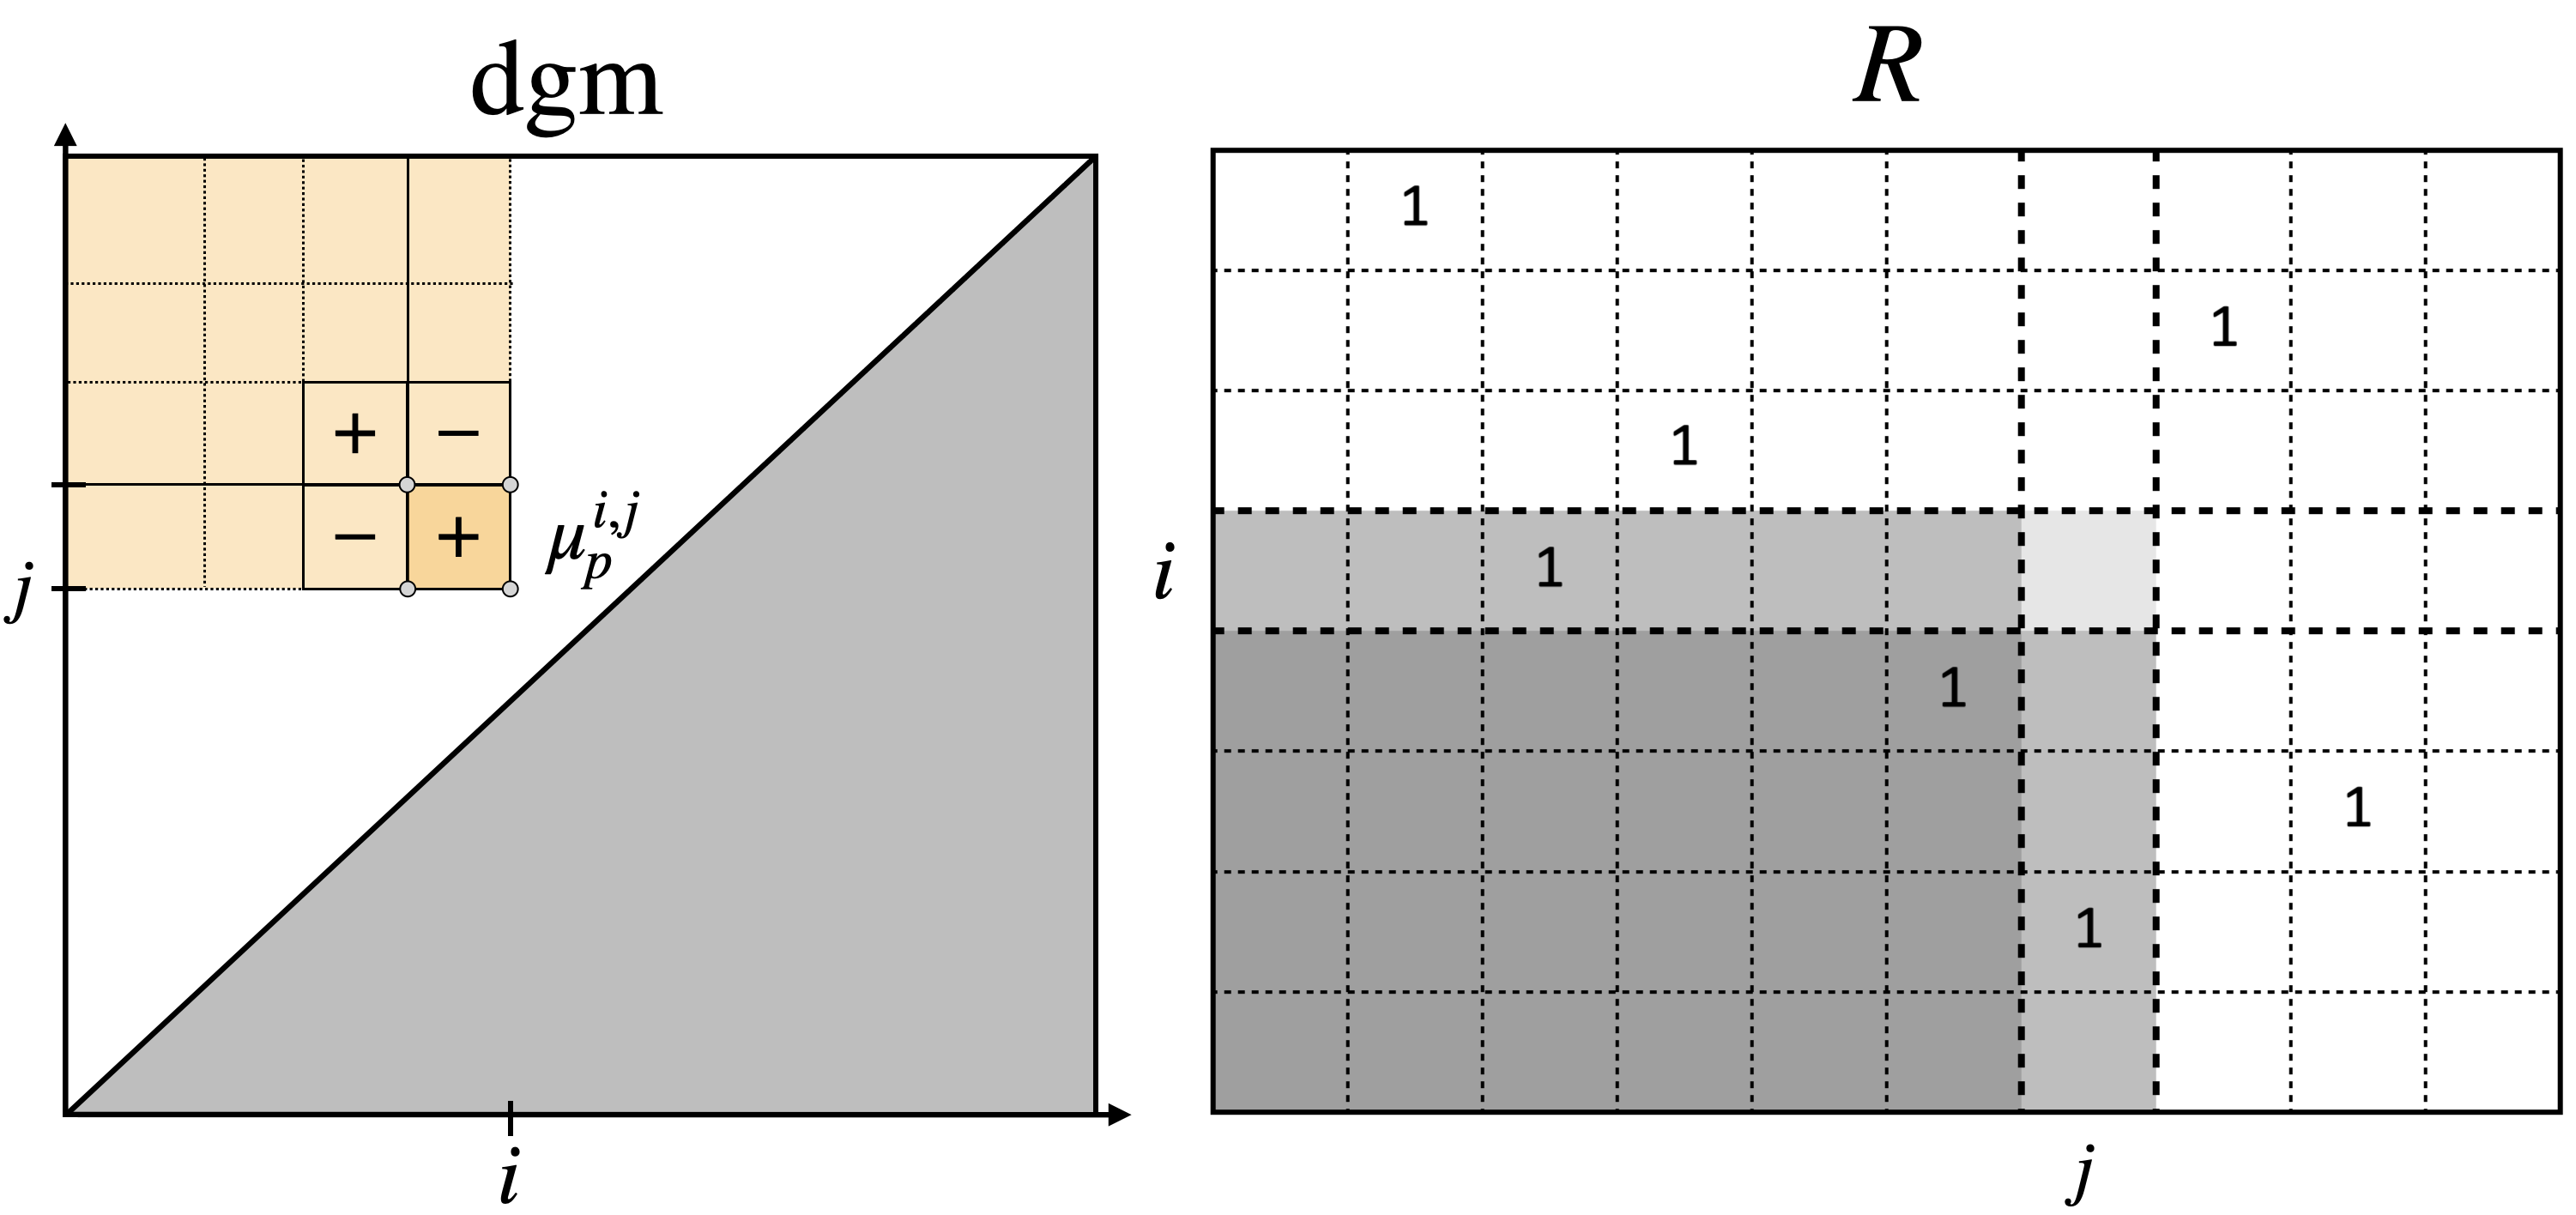
\includegraphics[width=0.45\textwidth]{mult_both}
	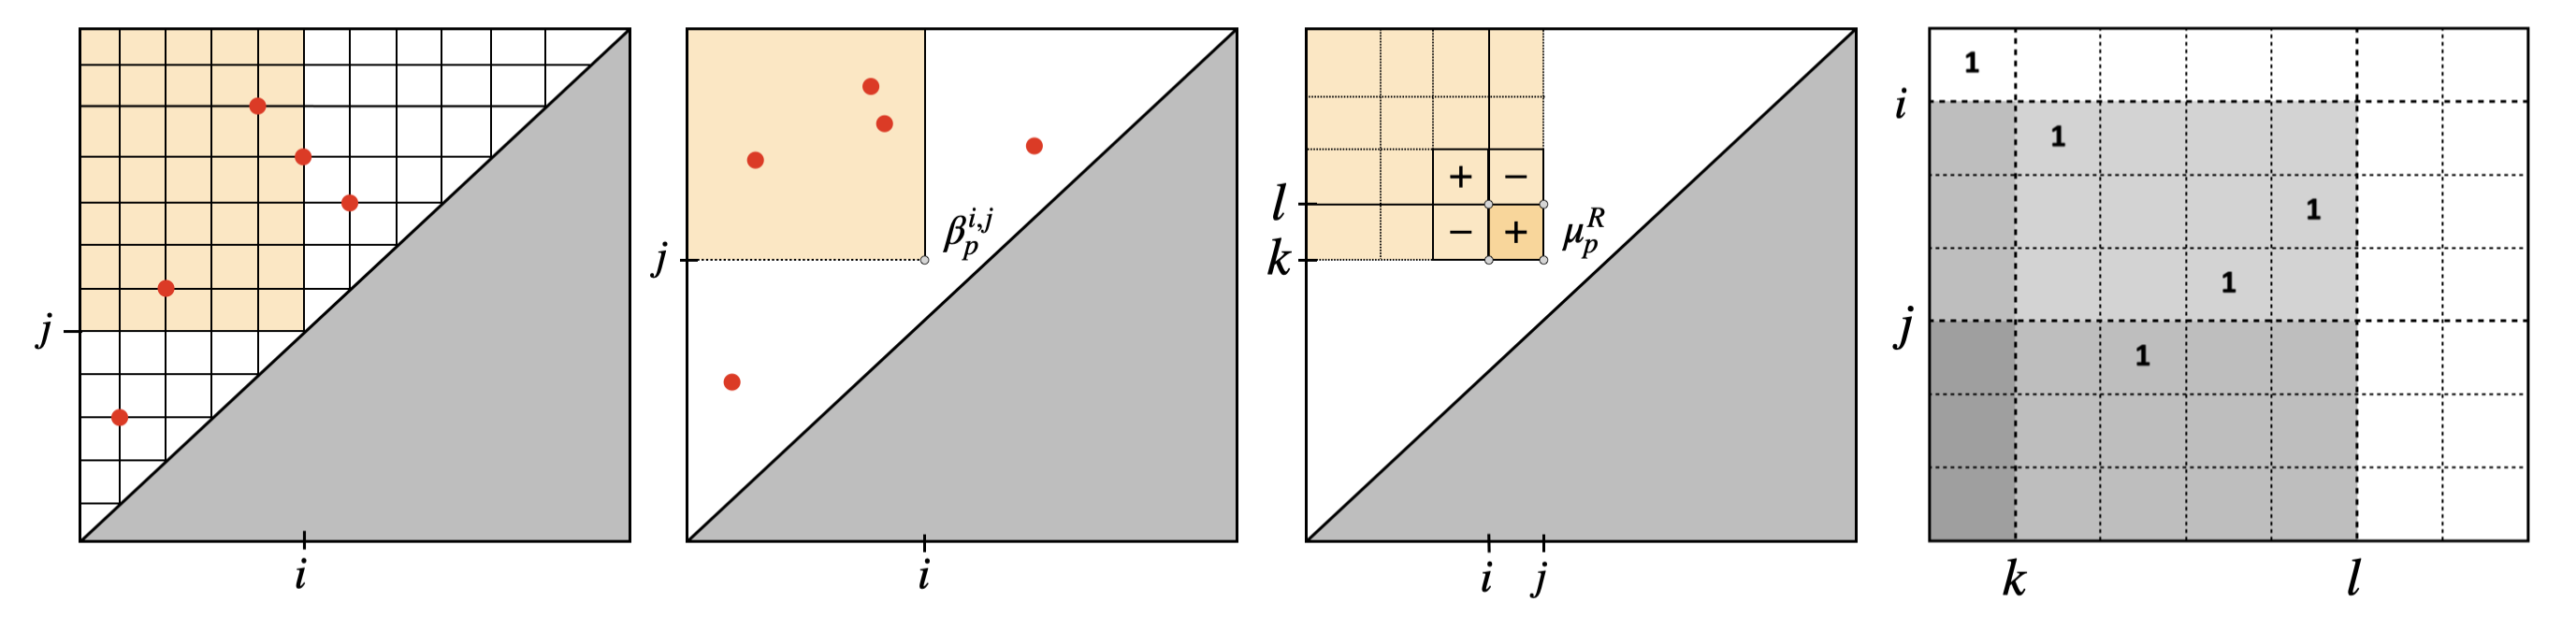
\includegraphics[width=0.85\textwidth]{betti_add}
	\caption{From left to right: $\beta_p^{i,j}$ counts the number of points (3) in upper left-corner of $\mathrm{dgm}_p(K_\bullet)$, where $i,j \in \Delta_+^m$; the same $\beta_p^{i,j}$  with $i,j \in \Delta_+$; the additivity of $\beta_p^{\ast}$ implies $\mu_p^{R}$ over a box $R=[i,j] \times [k,l]$ is given as the sum of four PBNs; generalization of the Pairing Uniqueness Lemma---in this case 	$\mu_p^R = 4 - 1 - 0 + 0 = 3$ counts pivot entries in the reduced matrix $R = \partial V$.}
	%$r_R(i,j) = 3 - 2 + 1 - 2 = 0$ yields whether the entry $R[i,j]$ is non-zero.}
	\label{fig:mult}
\end{figure}
For any $1 \leq i < j \leq m$, define the quantity $r_A(i,j)$ as follows:
\begin{equation}
	r_A(i,j) = \mathrm{rank}(A^{i,j}) - \mathrm{rank}(A^{i\texttt{+}1,j}) + \mathrm{rank}(A^{i\texttt{+}1,j\text{-}1}) - \mathrm{rank}(A^{i,j\text{-}1})
\end{equation}
%\begin{equation}
%	r_A(i,j) = \mathrm{rank}(A^{i, j}) - \mathrm{rank}(A^{i+1, j}) + \mathrm{rank}(A^{i+1, j-1}) - \mathrm{rank}(A^{i, j-1})
%\end{equation}
The structure theorem from~\cite{zomorodian2004computing} shows that 1-parameter persistence modules can be decomposed in an \emph{essentially unique} way into indecomposables. Computationally, a consequence of this phenomenon is the Pairing Uniqueness Lemma~\cite{cohen2006vines}, which asserts that if $R = \partial V$ is the decomposition of the boundary matrix, then:  
$$ r_R(i,j) \neq 0 \Leftrightarrow R[i,j] \neq 0 $$
Since the persistence diagram is derived completely from $R$, this suggests that information about a diagram can be obtained through rank computations alone.
For a more geometric description of this idea, see the third picture in Figure~\ref{fig:mult}. We record a non-trivial fact that follows from this observation: 
\begin{lemma}[Dey \& Wang~\cite{dey2022computational}]\label{lemma:rank}
Let $R = \partial V$ denote the matrix decomposition of a given filtered boundary matrix $\partial$ derived from the associated filtration $K_\bullet$. For any pair $(i,j)$ satisfying $1 \leq i < j \leq m$, we have:
	\begin{equation}\label{eq:lower_left_rank}
		\mathrm{rank}(R^{i,j}) = \mathrm{rank}(\partial^{i, j})
	\end{equation}
Equivalently, all lower-left submatrices of $\partial$ have the same rank as their corresponding submatrices in $R$. 
\end{lemma}
\noindent \textbf{Remark: } Though Lemma~\ref{lemma:rank} is defined over the full boundary matrix $\partial$, there is no loss in generality in extending this lemma to $p$-dimensional homology, for any fixed $p \geq 0$. To see this, note that since the reduction algorithm only adds $p$-chains to $p$-chains. Hence, if we set all columns corresponding to simplices of dimension $q \neq p$ to $0$ in the $m \times m$ boundary matrix $\partial$, then $\partial$ recovers the $p$-th boundary operator $\partial_p : C_p(K_\bullet) \to C_{p-1}(K_\bullet)$. 
In what follows, we will use $\partial_p$ and $R_p$ to refer to matrices of $\partial$ and $R$ whose $q$-chains are set to $0$, for $q \neq p $. 

Lemma~\ref{lemma:rank} was the essential motivating step used by Chen et al~\cite{chen2011output} in their rank-based persistence algorithm---the first output-sensitive algorithm given for computing persistent homology of a filtered complex.
The first fact we prove is that Lemma~\ref{lemma:rank} may be used to write the persistent Betti number as a sum of rank functions. 
\begin{proposition}\label{prop:rank_reduction}
Given a fixed $p \geq 0$, a filtration $K_\bullet$ of size $m = \lvert K_\bullet \rvert$, and any pair $(i,j) \in \Delta_+^m$, the persistent Betti number $\beta_p^{i,j}(K_\bullet)$ at $(i,j)$ is given by:
	\begin{equation}\label{eq:betti_four}
	% \mathrm{rank}(I_p^{1,i})
	\beta_p^{i,j}(K_\bullet) = i - \mathrm{rank}(\partial_p^{1,i}) - \mathrm{rank}(\partial_{p\+1 }^{1,j}) + \mathrm{rank}(\partial_{p\+1}^{i \+ 1, j} )
	%\mathrm{rank}(\partial_{p+1}^{i+1,\ast} \otimes\partial_{p+1}^{\ast,j} )
	\end{equation}
%where $I_p^{1,i}$ denotes the first $i$ columns of the $n \times n$ identity matrix.
\end{proposition}
\noindent A detailed proof of Proposition~\ref{prop:rank_reduction} is given in the appendix. It turns out Lemma~\ref{lemma:rank} can also be used to generalize~\eqref{eq:betti_four} to arbitrary rectangles in $\Delta_+$ via $\mu$\emph{-queries}: box-parameterized rank queries which count the number of persistence pairs that intersect a fixed ``box'' placed in the upper half-plane~\cite{chen2011output}. 
As a result, the $p$-th multiplicity function can also be defined in a rank-based formulation akin to~\eqref{eq:betti_four}. 
\begin{proposition}[Chen \& Kerber~\cite{chen2011output}]\label{prop:mu_reduction}
Given a fixed $p \geq 0$, a filtration $K_\bullet$ of size $m = \lvert K \rvert$, and a $R = [i,j] \times [k,l]$ whose indices $(i,j,k,l)$ satisfy $0 \leq i < j \leq k < l \leq m$, the $p$-th multiplicity $\mu_p^{R}$ of $K_\bullet$ is given by:
	\begin{equation}\label{eq:mu_four}
	\mu_p^{R}(K_\bullet) = \mathrm{rank}(\partial_{p\+1}^{j \+ 1, k})  - \mathrm{rank}(\partial_{p\+1}^{i \+ 1, k})  - \mathrm{rank}(\partial_{p\+1}^{j \+ 1, l}) + \mathrm{rank}(\partial_{p\+1}^{i \+ 1, l}) 
	%\mathrm{rank}(\partial_{p+1}^{i+1,\ast} \otimes\partial_{p+1}^{\ast,j} )
	\end{equation}
\end{proposition}
\noindent In summary, the complexity of computing either $\beta_p^{i,j}(K_\bullet)$ or $\mu_p^{R}(K_\bullet)$ can be reduced to the complexity of computing the rank of a set of ``lower-left'' submatrices of $\partial$. We summarize this fact with two corollaries.
\begin{corollary}
	Given a filtration $K_\bullet$ of size $m = \lvert K_\bullet \rvert$ and indices $i,j \in \Delta_+^m$, computing $\beta_p^{i,j}$ using expression~\eqref{eq:betti_four} requires $O(\mathrm{R}_{p}(j))$ time, where $\mathrm{R}_p(k)$ denotes the complexity of computing the rank of square $k \times k$ matrix with $O((p+2)k)$ non-zero $\mathbb{F}$ entries. 
	%$O(\mathrm{R}_p(n, i, p), \, R_\partial(m, j, p+1) \,\})$ where $R_\partial(a,b,c)$ is the complexity of computing the rank of a $c$-dimensional $a\times b$ boundary matrix with $b\cdot (c+1)$ non-zero $\mathbb{F}$ entries. 
	%with $n < m$
\end{corollary} 
\noindent Observe the relation $\partial_{p\+1}^{i \+ 1, j} \subseteq \partial_{p\+1}^{1, j}$ implies the  dominant cost of computing~\eqref{eq:betti_four} lies in computing either $\mathrm{rank}(\partial_p^{1,i})$ or $\mathrm{rank}(\partial_{p+1}^{1,j})$. As a result, we obtain a tighter bound for computing $\mu_p^R$ that is localized to the pair $(K_i, K_l)$. 
\begin{corollary}
	Given a filtration $K_\bullet$ of size $m = \lvert K_\bullet \rvert$ and a rectangle $R = [i,j] \times [k,l]$ with indices $0 \leq i < j \leq k < l \leq m$, computing $\mu_p^{R}$ using expression~\eqref{eq:mu_four} requires $O(\mathrm{R}_{p}(l - i))$ time, where $\mathrm{R}_p(k)$ denotes the complexity of computing the rank of square $k \times k$ matrix with $O((p+2)k)$ non-zero $\mathbb{F}$ entries.
	%$ j(p+1) - i$
	%time and storage complexity $O(\max \{\, R_\partial(n, i, p), \, R_\partial(m, j, p+1) \,\})$ where $R_\partial(a,b,c)$ is the complexity of computing the rank of a $c$-dimensional $a\times b$ boundary matrix with $b\cdot (c+1)$ non-zero $\mathbb{F}$ entries. 
	%with $n < m$
\end{corollary} 

\noindent Compared to other classical methods of obtaining $\beta_p^{\ast}(K_\bullet)$ and $\mu_p^\ast(K_\bullet)$, such as those in~\cite{edelsbrunner2022computational, zomorodian2004computing}, the primary advantage the rank-based expressions from~\eqref{eq:betti_four}-\eqref{eq:mu_four} have is that their computations are performed directly on \emph{unfactored} boundary matrices. 
We dedicate the rest of the paper to exploring the consequences of this fact. 

%We exploit various properties of the rank function to 
%Using various properties of the rank function, this accelerate the computation of both invariants. 
%Combined with various properties of the rank function, we exploit this aspect of to accelerate the computation of both invariants in~\eqref{eq:betti_four} and~\eqref{eq:mu_four}. 

%To get some intuition on what the structure and size of these matrices, we include a picture of each of the terms in Equation~\eqref{eq:betti_four}. 
%\begin{figure}[!h]
%	\centering
%	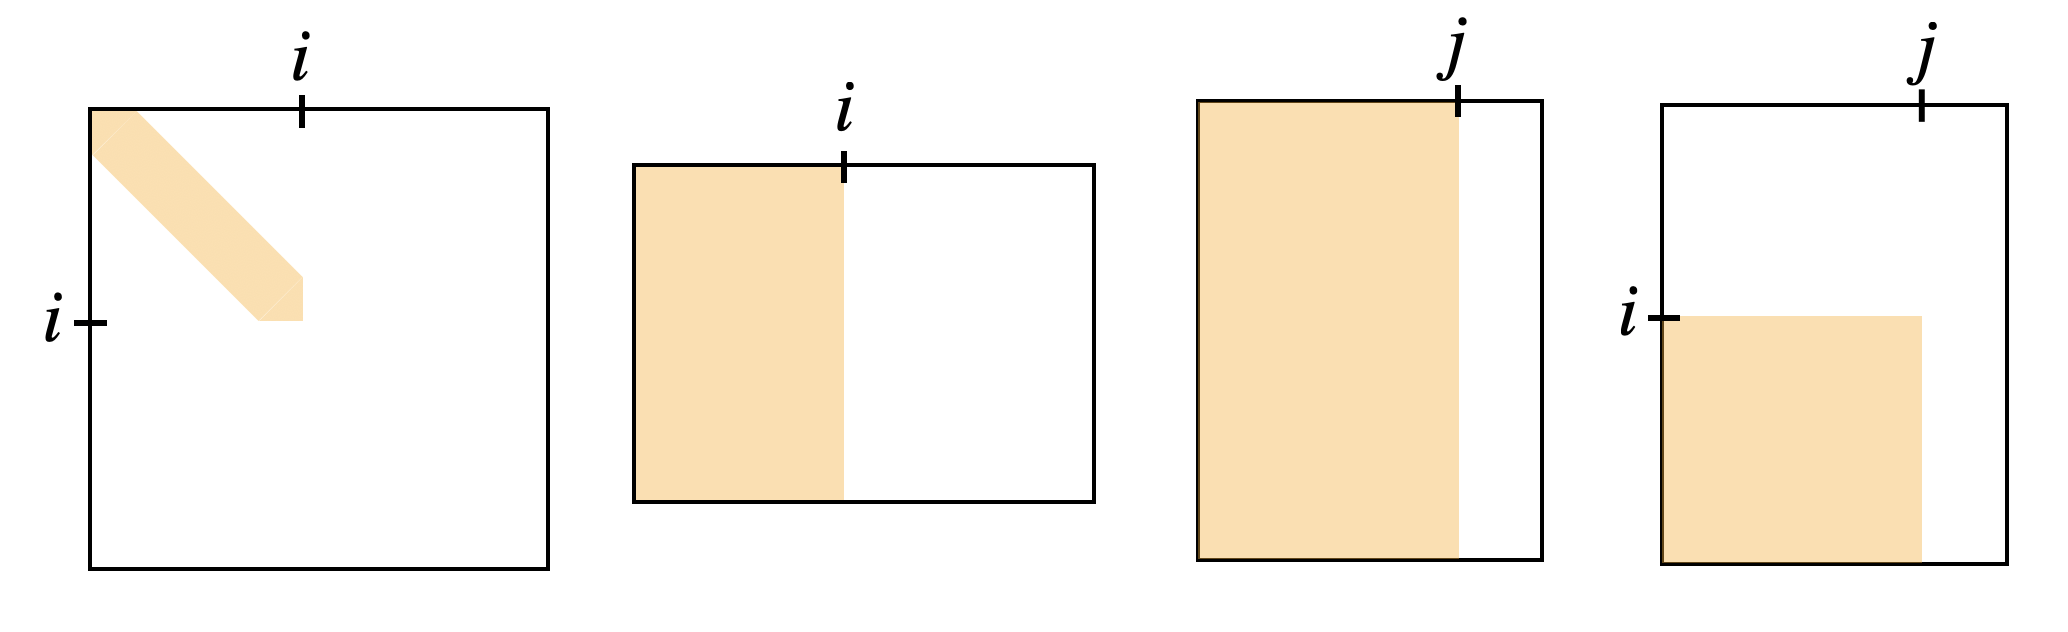
\includegraphics[width=0.70\textwidth]{four_matrices}
%	\caption{The four matrices whose ranks yield $\beta_p^{i,j}$ in the same order as given in~\eqref{eq:betti_four}. Each solid portion represents (sparse) blocks of non-zero entries, while each white portion is zero. Observe $\partial_{p+1}^{i+1, j} \subseteq \partial_{p+1}^{1,j}$ can be obtained by intersecting the non-zero entries of $\partial_{p+1}^{1,j}$ with the non-zero entries in the complement of $\partial_p^{1,i}$.  }
%\end{figure}
%Boundary matrices are sparse and highly structured: given $K_\bullet$ with $m$ simplices $\sigma_1, \sigma_2, \dots, \sigma_m$ constructed from a $p$-dimensional complex $K$, its full boundary matrix $\partial$ is upper-triangular and has a storage complexity of: 
%\begin{equation}
%	\mathrm{nnz}(\partial) \sim O(m \log m)
%\end{equation} 
%To see this, note that since a $p$-simplex has $2^{p+1} - 1$ faces, we have $p \leq \log(m + 1) - 1$. Moreover, since each column of $\partial_p^\ast$ contains exactly $p+1$ non-zero entries, $\mathrm{nnz}(\partial) \sim O((p+1)m)$.


%\begin{proposition}\label{prop:mu_query}
%For any fixed $p \geq 0$, let $\partial_p$ denote the $p$-dimensional boundary matrices of filtration $K_\bullet$ of size $n = \lvert K^{(p)} \rvert$, $m = \lvert K^{(p\+1)} \rvert$.
%Let $R = [i,j] \times [k,l]$ denote a fixed rectangle in $\mathbb{R}^2$ satisfying $a < b \leq c < d$. The multiplicity $\mu_p^R$ of this box is given by:
%	\begin{equation}\label{eq:mu_four}
%	\mu_p^{R} =  \mathrm{rank}(\partial_{p\+1}^{j} ) - \mathrm{rank}(\partial_{p\+1}^{i \+ 1, j} )
%	%\mathrm{rank}(\partial_{p+1}^{i+1,\ast} \otimes\partial_{p+1}^{\ast,j} )
%	\end{equation}
%where $I_p^{1,i}$ denotes the first $i$ columns of the $n \times n$ identity matrix.
%\end{proposition}
%\begin{corollary}
%	Given a filtration $K_\bullet$ of size $n = \lvert K_{i}^{(p)} \rvert$ and $m = \lvert K_{j}^{(p+1)} \rvert$ and two indices $i \in [n]$, $j \in [m]$, computing $\beta_p^{i,j}$ can be done in time and storage complexity $O(\max \{\, R_\partial(n, i, p), \, R_\partial(m, j, p+1) \,\})$ where $R_\partial(a,b,c)$ is the complexity of computing the rank of a $c$-dimensional $a\times b$ boundary matrix with $b\cdot (c+1)$ non-zero $\mathbb{F}$ entries. 
%	%with $n < m$
%\end{corollary} 

% This subsection shows the benefits of rank(P^T A P) = rank(A)
\subsection{A Parameterized Boundary Matrix Relaxation}
Expressing the PBN via~\eqref{eq:betti_four} enables us to exploit properties of the rank function which are advantageous in \emph{parameterized} settings, i.e. settings where the input data is  thought to be generated from a parameterized family.  
One such property is permutation invariance: given any $A \in \mathbb{R}^{n \times n}$, it is well known that $\mathrm{rank}(A) = \mathrm{rank}(P^T A P)$ for any permutation matrix $P$. Though  the boundary matrices $\partial_p$ in~\eqref{eq:betti_four} are given in filtration order to elucidate their structure, the permutation invariance of the rank function suggests they need not be in such an order to be evaluated---so long as the constitutive terms have the same non-zero pattern as their filtration-ordered counterparts, their ranks and thus their PBNs will be identical.
In what follows, we re-define the boundary matrix to exploit this permutation invariance. 
 
%% Another approach to tracking the PBNs in parameterized setting is to maintain a persistence diagram through the vineyards algorithm~\cite{cohen2006vines}. This, however, requires $O(m^2)$ memory and an $\approx O(m^2)$ preprocessing procedure to detect changes in the filtration order\footnote{The bound $O(m^2)$ assumes the homotopy changes each filtration value monotonically throughout the homotopy. Otherwise the number of order changes is clearly unbounded.} to simulate persistence across a homotopy, the canonical continuous parameterized setting. In contrast, as we show below, PBNs need no such preprocessing procedure and may be computed in effectively $O(m)$ memory, even in parameterized settings. 
%Recall that the boundary operator $\partial_p$ for a filtration pair $(K_{\bullet}, f)$ of size $m = \lvert K \rvert$ is represented by an ordered $(m \times m)$ boundary matrix $\partial_p$ whose columns and rows corresponding to $q$-simplices and $(q-1)$-simplices are zero, for $q \neq p$.
%After orienting $K$ in an arbitrary but consistent way, the entries of $\partial_p$ have the form: 
%\begin{equation}\label{eq:matrix_pchain}
%	\partial_p[k, l] = \begin{cases} 
%	c(\sigma_j)  & \text{if } \sigma_l \in \partial_p(\sigma_k) \\
%	0 & \text{otherwise}
%   \end{cases}
%\end{equation}
%where $c(\sigma_\ast) \in \mathbb{F}$ is an arbitrary constant satisfying $c(\sigma) = -c(\sigma')$ if $\sigma$ and $\sigma'$ are opposite orientations of the same simplex, typically set to $\pm 1$. In what follows, we assume a fixed orientation is given on $K$, and write $\pm c(\sigma)$ to indicate the sign of $c(\sigma)$ depends on the orientation of $\sigma$. Note that, for the reduction algorithm, the ordering of $\partial_p$ must respect the facet poset of $K_\bullet$: if $\tau, \sigma \in K_\bullet^{(p)}$ and $f(\tau) \leq f(\sigma)$, then the chain $\partial_p(\tau)$ must appear before $\partial_p(\sigma)$ in $\partial_p$. %such that the elementary left-to-right matrix operations. 

% Change index set
All of the notation given thus far, such as the definitions of the PH groups~\eqref{eq:hom_map} and the the PBN~\eqref{eq:pbn}, have used integer indices $(i,j) \in \Delta_+^m$ to describe the PH groups over a filtration pair $(K_\bullet, f)$ of size $\lvert K \rvert = m$. Equivalently, we have thus far implicitly assumed the range of the filter function $f : K \to I$ to be the typical index set $I = [m]$.
In practice, the filter function $f$ is often derived from geometrical settings wherein it is more informative to interpret the persistence of a persistent-pair $(\sigma_i, \sigma_j) \in \mathrm{dgm}(K_\bullet)$ as $f(\sigma_j) - f(\tau_i)$, rather than as $j - i$, as the filter function $f : K \to \mathbb{R}$ is quite often real-valued.
% In theory, any function satisfying $f(\tau) \subseteq f(\sigma)$ for every face/coface pair $(\tau, \sigma)$ yields a well defined persistence diagram. 
In what follows, in the spirit of~\eqref{eq:pbn_cont}, we alter our notation by re-defining $\beta_p^{i,j}$ using pairs $(i,j) \in \Delta_{+}$ from the upper-half plane $\Delta_{+} = \{ (x,y) \in \mathbb{R}^2 : y > x \} $.

%such that $\mathrm{range}(f) = \mathbb{R}$, and it is often more informative to work with the pairs $(f(\tau_i), f(\sigma_j))$ stemming from the persistent-pairs $()$ persistence diagram 
% A common scenario is where $K_\bullet$ is obtained via a Rips filtration constructed over a metric space $(X, d_X)$. In this case $f : \mathcal{P}(X) \to \mathbb{R}_+$ is given as the diameter $f(\sigma) = \max_{x,x' \in \sigma} d_X(x,x')$. 
% mention DMSs 
%In many applications it is of interest to study such filter function in parameterized settings, e.g. given some set of parameters $\mathcal{H}$, the goal is to understand a given topological invariant at many  parameters $h \in \mathcal{H}$, i.e. treat $f : \mathcal{P}(X) \times \mathcal{H} \to \mathbb{R}_+$. We include several example in section~\ref{}.

Suppose that instead of being given a fixed pair $(K_\bullet, f)$, the filter function was parameterized $f : \mathcal{H} \times K \to \mathbb{R}$ and one was interested in computing $\beta_p^{i,j}$ over $\mathcal{H}$. We give several application contexts where this kind of formulation occurs naturally in section~\ref{sec:applications}. As a first step to simplifying the PBN computation in this setting, we introduce the notion of a \emph{parameterized boundary matrix}.
% $\delta_{\mathcal{X}}(\cdot) = (X, d_X(\cdot))$ a DMS over a finite set $X$ of fixed size $\lvert X \rvert = n$
% TODO: fix i,j to be [n], [m]... no need for upper half plane yet 
\begin{definition}[Parameterized boundary matrix]\label{def:time_boundary_matrix}
Let $K$ denote an abstract simplicial complex of size $\lvert K \rvert = m$, equipped with parameterized filtering function $f : K \times \mathcal{H} \to \mathbb{R}$. 
Assume $K$ is ordered along a fixed but arbitrary linear extension $(K, \preceq^\ast)$ of the face poset of $K$. For fixed $(i,j) \in \Delta_{+}$, define the $\mathcal{H}$-\emph{parameterized} $p$\emph{-th boundary matrix} $\hat{\partial}_p^{i, j}(h)$ \emph{at scale} $(i,j)$ to be the $m \times m$ matrix ordered by $\preceq^\ast$ for all $h \in \mathcal{H}$, and whose entries $(k,l)$ satisfy:
\begin{equation}\label{eq:param_boundary_matrix}
	\hat{\partial}_p^{i,j}(h)[k,l] = \begin{cases}
	% \pm \, S_{i,j}(\sigma_k, \sigma_l) & \text{if } \sigma_k \in \partial_p(\sigma_l) \\
	\pm \, (S_{i} \circ f_h)(\sigma_k) \cdot (\tilde{S}_{j} \circ f_h)(\sigma_l) & \text{if } \sigma_k \in \partial_p(\sigma_l) \\
	%, \text{ where } \epsilon = f(\sigma_l) \\
	0 & \text{otherwise}
\end{cases}
\end{equation}
% where $S_{\omega}^{\alpha} : \mathbb{R} \to [0, 1]$ is a \emph{smooth-step} function whose range decreases smoothly from $1 \to 0$ in the interval $[\alpha - \omega, \alpha]$.
%where $S_{i, j} : \mathcal{P}(X) \times \mathcal{P}(X) \to \{0, 1\}$ is a \emph{step} function that accepts a face/coface pair $(\sigma_k, \sigma_l)$ and returns a $1$ if $f(\sigma_k) \geq i$ and $f(\sigma_l) \leq j$, and $0$ otherwise. 
where $S_{i} : \mathbb{R} \to \{0, 1\}$ is a \emph{step} function satisfying $S_i(x) = 0$ if $x \leq i$ and $1$ otherwise, $\tilde{S}_{i} = 1 - S_i$, and $f_h(\sigma) = f(\sigma, h)$.
\end{definition}
\noindent
We now show definition~\ref{def:time_boundary_matrix} simplifies the expression of the PBN in parameterized settings. To simplify the notation, we write $A^{x} = A^{\ast,x}$ for the setting where only columns up to $x$ of $A$ are being selected, and let $q = p + 1$. 
%We also write $r(A) = \mathrm{rank}(A)$.
% TODO: ask Jose about this
%We also use $\mathcal{K}_f$ to denote the space of all filtration pairs $(K, f)$.
Let $V = \{ v_1, v_2, \dots, v_n\}$ denote a fixed vertex set. The parameterized PBN can be written as: 
\begin{align*}\label{eq:pbn_parameterized}
	\beta_p^{i,j} : \mathcal{H} \times \mathcal{P}(V) &\to \mathbb{N} \\
	%h &\mapsto \lvert K_i^{(p)}(h) \rvert  -  (\mathrm{r} \circ \hat{\partial}_{p}^{i})(h) - (\mathrm{r} \circ \hat{\partial}_{q}^{j})(h) + (\mathrm{r} \circ \hat{\partial}_{q}^{i \+ \epsilon, j})(h) \numberthis
	h, K &\mapsto \lvert K_i^{(p)}(h) \rvert - \mathrm{rank}\big(\,\hat{\partial}_{p}^{i}(h)\,\big) - \mathrm{rank}\big(\,\hat{\partial}_{q}^{j}(h)\,\big) + \mathrm{rank}\big(\,\hat{\partial}_{q}^{i \+ \epsilon, j}(h)\,\big) \numberthis
\end{align*}
% deflation?
where $\epsilon > 0$ is an arbitrarily small positive number. Observe~\eqref{eq:pbn_parameterized} is essentially the same form as~\eqref{eq:betti_four}. 
By Proposition~\ref{prop:mu_reduction}, we also have a parameterized multiplicity function for any rectangle $R = [i,j] \times [k,l]$ in the upper half-plane $\Delta_{+}$ satisfying $i < j \leq k < l$: 
\begin{align*}\label{eq:mu_parameterized}
	\mu_p^{R} : \mathcal{H} \times \mathcal{P}(V) &\to \mathbb{N} \\
	h, K & \mapsto  \mathrm{rank}\big(\,\hat{\partial}_{q}^{j \+ \epsilon, k}(h)\,\big) - \mathrm{rank}\big(\,\hat{\partial}_{q}^{i \+ \epsilon, k}(h)\,\big) - \mathrm{rank}\big(\,\hat{\partial}_{q}^{j \+ \epsilon, l}(h)\,\big) + \mathrm{rank}\big(\, \hat{\partial}_{q}^{i \+ \epsilon, l}(h)\,\big) \numberthis
\end{align*}


%One remark is in order: note that although definition~\ref{def:time_boundary_matrix} specifies $\hat{\partial}_p^{i,j}$ as a full $\binom{n}{p} \times \binom{n}{q}$ matrix, implying a memory complexity of $O(q\cdot n^{q})$ for all $h \in \mathcal{H}$, we remark that there is no need to fully allocate this much memory as the rows/columns corresponding to the set of $p$/$q$ face/coface pairs $(\sigma_k, \sigma_l)$ with $f(\sigma_l) < i$ or $f(\sigma_k) > j$ are entirely $0$. 
%As we will show below, it is enough to have access to the simplices $K_j^{(q)}(h)$. % and $\bar{K}_i^{(p)}(h)$?

% In general, computing dgm_p(X) for p \geq 1 requires O(\lvert X \rvert^{3(p+2)}) [ p = 1 <=> O(n^9), p=2 <=> O(n^12)] (curvature sets paper) and O(\lvert X \rvert^{2(p+2)}) memory.

% Benefits of rank(A) = rank(A^T A) = rank(A A^T)


%\subsection{Special Cases} The spectrum of the graph Laplacian is known to have closed-form expressions for certain structured graphs. In particular, the spectra of the cycle graph $C_n$ and the path graph $P_n$ over $n$ vertices is given by: 
%\begin{equation}
%	\Lambda(C_n) = 1-\cos\left (\frac{2\pi k}{n} \right), \quad \Lambda(P_n) = 1-\cos\left (\frac{\pi k}{n-1} \right)
%\end{equation}
%for all $k = 0, 1, \dots, n-1$. Thus, if we know ahead of times the graph we are working with is one of these special graphs, it follows that may read off its $(i,j)$-th PBN in $O(n)$ time. 

%Moreover, by composing the vertex and edge functions $f_V$ and $f_E$, respectively, with the step functions $S_\ast : \mathbb{R} \to \{0, 1\}$

%graph has a unique Laplacian matrix, this matrix does not in general uniqueIy
%determine a graph: the Laplacian tells us nothing about how many Ioops were
%to be found in the original graph.
% The characteristic polynomial of L(G) is given as the product of the characteristic polynomial of its disjoint subgraphs L(G_1), ..., L(G_k).
% The Spectrum of the Laplacian in Riemannian 	Geometry
% The spectrum does not in general determine the geometry of a manifold. Nevertheless, some geometric information can be extracted from the spectrum. In what follows, we define a spectral invariant to be anything that is completely determined by the spectrum






% TODO: UNDERSTAND THE FOURTH TERM 
%The graph laplacian appears naturally in the computation of $\beta_0^\ast$. Consider the rank expression from~\eqref{eq:betti_four}. Since $\partial_0$ is trivial, the expression reduces to: 
%\begin{equation}
%	\beta_p^{i,j} = \lvert K_i^{(0)}\rvert - \mathrm{rank}(\partial_{1}^{j}) + \mathrm{rank}(\partial_{1}^{i \+ 1, j} )
%\end{equation} 
%Since $\mathrm{rank}(A) = \mathrm{rank}(A A^T) = \mathrm{rank}(A^T A)$, we may equivalently express the second and third terms in terms of their graph Laplacians. Let $G_j = \mathcal{L}(K_j)$ denote the graph of $K_j$...
%as $\mathrm{rank}(L(K_j))$ and $\mathrm{rank}(L(K_j \cap \bar{K}_i))$, where $\bar{K}_i = K_\bullet \setminus K_i$ denotes the complement. Since the rank of any (irreducible) graph Laplacian may be deduced by counting the connected components of the underlying graph, we deduce that the complexity of computing $\beta_0^{i,j}$ reduces to the complexity 
% TODO: compute this for small example to verify Laplacians

%\textbf{Example:} Consider a 2-simplex $K = \Delta_2$ with vertex weights $\mathrm{Im}(f_E) = \{a, b, c\}$ and edge weights $\mathrm{Im}(f_E) = \{d,e,f\}$. Suppose we augment the chain expressions in boundary matrix $\partial_p$ to reflect The matrix representations of 


%For $p \geq 1$, the PBN expression can still be generalized via \emph{up Laplacians}. The higher-dimensional generalizations of the graph Laplacian for simplicial complexes have been studied in a variety of settings, see e.g.~\cite{}. 
%In particular, given $K$ a finite oriented simplicial complex and some $p \geq 0$, the $p$-th \emph{combinatorial Laplacian} of $K$ is the linear operator $\mathcal{L}_p : C_p \to C_p$ given by: 
%\begin{equation}
%	\mathcal{L}_p = \partial_{p\+1} \circ \partial_{p\+1}^T + \partial_{p}^T \circ \partial_{p}
%\end{equation}
%For convenience, we use the notation ${\uparrow}L_p = \partial_{p\+1} \circ \partial_{p\+1}^T$ and ${\downarrow}L_{p} = \partial_{p}^T \circ \partial_{p}$ to denote the so-called \emph{up} and \emph{down} combinatorial $p$-th Laplacians, respectively. 
%With this notation, notice the computation of the PBN can be expressed via the ranks of up Laplacians...

%We now show a few properties that the rank-based formula $\beta_p^{i,j}$ exhibits that are advantageous in parameterized settings. 
%The first such property is a simple parameterized relaxation of PBN:
%\begin{align*}
%	\hat{\beta}_p^{i,j} &= \lvert K_i^{(p)} \rvert - \mathrm{rank}(\partial_{p}^{i}) - \mathrm{rank}(\partial_{q}^{j}) + \mathrm{rank}(\partial_{q}^{i \+ 1, j} ) \\
%%	&= \lvert K_i^{(p)} \rvert - \mathrm{rank}((\partial_{p}^{i})(\partial_{p}^{i})^T) - \mathrm{rank}(\underbrace{(\partial_{q}^{j})(\partial_{q}^{j})^T}_{\uparrow\mathcal{L}_1^i}) + \mathrm{rank}((\partial_{q}^{i \+ 1, j})(\partial_{q}^{i \+ 1, j})^T)
%&= \lvert K_i^{(p)} \rvert - \mathrm{rank}((\partial_{p}^{i})(\partial_{p}^{i})^T) - \mathrm{rank}((\partial_{q}^{j})(\partial_{q}^{j})^T) + \mathrm{rank}( (\partial_{q}^{i \+ 1, j})(\partial_{q}^{i \+ 1, j})^T)\\
%&= \lvert K_i^{(p)} \rvert - \mathrm{rank}(L_p^i) - \mathrm{rank}(L_q^j) + \mathrm{rank}(L_q^{i\+1,j}) \numberthis
%\end{align*}

% \hat{\beta}_p^{i,j} = \sum\limits_{\underset{\lvert \sigma \rvert = p+1}{\sigma \in \mathcal{P}(X)}} \mathrm{sgn}\left( \; \lvert i - f(\sigma) \rvert_{\+} \right)  - \mathrm{rank}(\partial_{p}^{i}) - \mathrm{rank}(\partial_{q}^{j}) + \mathrm{rank}(\partial_{q}^{i \+ 1, j} )

%Clearly the entries of $\partial_p(t)$ now vary smoothly in $t \in T$. Moreover, for fixed $p \geq 0$, we have:
%\begin{enumerate}
%	\item $\mathrm{rank}(\partial_p^t) = \mathrm{dim}(\mathrm{B}_{p-1}(K_t))$ for all $t \in T$ 
%	\item $\lVert \partial_p^t - \partial_p^{t'} \rVert_F \sim O(m_p)$ when $\delta_\mathcal{X}$ is $C$-Lipshitz over $T$ and $\lvert t - t' \rvert$ is small,
%	\item $\lVert \partial_p^t \rVert_{2} \leq \epsilon \sqrt{\kappa} \, (p+1)$ where $\kappa = \max \sum\limits_{t \in T}\sum\limits_{\sigma \in K_t}\mathds{1}(\mathrm{diam}(\sigma) \leq \epsilon)$
%	%\sqrt{\epsilon\,\kappa\,(p+1)}$ where $\kappa = \max \sum\limits_{t \in T}\sum\limits_{\sigma \in K_t}\mathds{1}(\mathrm{diam}(\sigma) \leq \epsilon)$ %$C(n,k) = \binom{n}{k}$
%\end{enumerate}

\subsection{Complexity of Persistence}
 

\section{Spectral PBN relaxation and its implications}\label{sec:methodology}
%\subsection*{An quadratic-time rank computation}
In this section we discuss the computational details involved in evaluating the rank function on the boundary matrices whose columns take the form~\eqref{eq:alt_sum}. We begin with a spectral characterization of the rank function. Given a matrix $X \in \mathbb{R}^{n \times m}$ and its singular value decomposition (SVD) $X = U \Sigma V^T$, define the \emph{rank} of $X$ as the composition:
%of the one-sided sign function with the singular value function:
\begin{equation}\label{eq:rank_def}
	\mathrm{rank}(X) = \sum\limits_{i=1}^{n} \mathrm{sgn}_+(\sigma_i(X)), \quad \quad \mathrm{sgn}_{+}(x) = \begin{cases}
		1 & \text{if } x > 0 \\
		0 & \text{otherwise}
	\end{cases}
\end{equation}
where $\Sigma = \mathrm{diag}(\{\sigma_1, \sigma_2, \dots, \sigma_n \})$ are the singular values  and $\mathrm{sgn}_+: \mathbb{R} \to \{0, 1\}$ is the one-sided sign function. As~\eqref{eq:rank_def} is defined completely in terms of the singular values of $X$, and the singular values of $X$ are given by the square roots of eigenvalues of $X X^T$ (or $X^T X$), we focus on iterative methods for finding the eigenvalues of Hermitian matrices. 
%In particular, we focus on the Lanczos iteration applied to positive semi-definite matrices, diagonally dominant (DD) and strictly diagonally dominant (SDD) matrices, and combinatorial Laplacians. We also show how these methods made be adapted to efficiently compute~\eqref{eq:pbn_parameterized} and~\eqref{eq:mu_parameterized}.

% Benefits of rank(A) = < non-zero eigenvalues >
\subsection{The Lanczos iteration}
% Summarized from "The Lanczos Method: Evolution and Application" 
For a real, square matrix $A$ of order $n$, the quadratic form $x^T A x$ defines a continuous real-valued function of $x \in \mathbb{R}^n$. When $A$ is symmetric positive definite, the implicit equation $x^T A x = 1$ defines an $n$-dimensional ellipsoid $y^T \Lambda y = 1$ whose $n$ principle axes are eigenvectors $\{v_i\}_{i=1}^n$ and whose lengths are the squares of eigenvalues $\Lambda(A)$ of $A$.
%i.e. $y^T \Lambda y = \lambda_1 y_1^2 + \lambda_2 y_2^2 + \dots + \lambda_n y_n^2$. 
Each eigen-pair $(\lambda, v)$ satisfies $A v = \lambda v$, and when $A$ is symmetric, every $\lambda$ is real-valued and every pair of eigenvectors $v, u \in \mathbb{R}^n$ whose corresponding eigenvalues $\lambda \neq \lambda'$ are orthogonal.  
% https://netlib.org/lanczos/vol2/Chp_2_RealSymmetric.pdf
Thus we may reveal the spectrum $\Lambda(A)$ of $A$---effectively the lengths of the aforementioned ellipsoid---via orthogonal diagonalization:
%by constructing an orthonormal eigenvector basis $V$ of $A$,
\begin{equation}\label{eq:eigen_decomp}
	A = V \Lambda V^T = \sum\limits_{i=1}^n \lambda_i v_i v_i^T
\end{equation}
% Insert similarity transforms  
Factorizing $A$ as in~\eqref{eq:eigen_decomp} is known as the \emph{symmetric eigenvalue problem}. 
Computing eigen decompositions of symmetric matrices generally consists of two phases: (1) reduction to tridiagonal form $Q^T A Q = T$ via orthogonal similarity transformations $Q = Q_1 Q_2 \dots Q_{n-2}$, and (2) diagonalization of the tridiagonal form $T = Y \Theta Y^T$. 
% For phase (2), also see: https://www.cs.utexas.edu/users/flame/laff/alaff-beta/chapter10-francis-implicit-qr-step.html
Note the latter may be performed in $O(n \log n)$ time~\cite{gu1995divide}, whereas the former is effectively bounded below by $\Omega(n^3)$ for dense full-rank matrices using non-Strassen-like operations, and thus this reduction to tridiagonal form dominates the computation. 
Lanczos~\cite{lanczos1950iteration} proposed the \emph{method of minimized iterations}---now known as the \emph{Lanczos method}---as an attractive alternative for reducing $A$ into a tridiagonal form and thus revealing its spectrum.
% Mention reflectors destroy sparsity 
% orthogonally diagonalizable 
%The eigen-decomposition of a symmetric $A$ not only produces an orthogonal basis for $A$, but for every $1 \leq r \leq \mathrm{rank}(A)$, the matrix $A_{(r)} = V_r \, \mathrm{diag}(\{\sigma_1, \dots, \sigma_r\}) \, V^T_r$ is the closest matrix to $A$ in the Frobenius norm: 
%\begin{equation}
%	A_{(r)} = \argmin_{B \in \mathbb{R}^{n \times n}}\lVert A - B \rVert_F
%\end{equation}
% History of Lanczos 
%The success of iterative methods at extracting spectral-information from large, sparse matrices in the past three decades is unprecedented. Core to these methods is what is known today as the Lanczos method~\cite{}, or as Lanczos called it, the \emph{method of minimized iterations}. Although discovered before the widely successful direct methods (Householder transformations, QR factorization, etc.), the Lanczos algorithm became the staple for applications where the underlying decomposition of system was too large to fit into memory. 
%We review the method briefly in what follows.
%reduces $A$ to tridiagonal form via a series of orthogonal similarity transformations
 
The means by which the Lanczos method estimates eigenvalues is by projecting onto successive Krylov subspaces. Given a large, sparse, symmetric $n \times n$ matrix $A$ with eigenvalues $\lambda_1 \geq \lambda_2 > \dots \geq \lambda_r > 0$ and a vector $v \neq 0$, the order-$j$ Krylov subspaces of the pair $(A, v)$ are the spaces spanned by: 
\begin{equation}
	\mathcal{K}_j(A, v) := \mathrm{span}\{ v, Av, A^2 v, \dots, A^{j-1} \} = \mathrm{range}(K_j(A, v))
\end{equation}
where $K_j(A, v) = [ v \mid Av \mid A^2 v \mid \dots \mid A^{j-1}]$ are their corresponding Krylov matrices. 
% The utility of Krylov subspace methods is motivated by the fact that the minimal polynomial of $A$ can be used to express $A^{-1}$ in terms of powers of $A$.
Krylov subspaces arise naturally from using the minimal polynomial of $A$ to express $A^{-1}$ in terms of powers of $A$. In particular, if $A$ is nonsingular and its minimal polynomial has degree $m$, then $A^{-1}v \in K_m(A, v)$ and $K_m(A, v)$ is an invariant subspace\footnote{Recall that if $S \subseteq \mathbb{R}^n$, then $S$ is called an \emph{invariant subspace} of $A$ or $A$-\emph{invariant} iff $x \in A \implies Ax \in S$ for all $x \in S$.} of $A$.
% "Krylov subspace methods for shifted unitary matrices and eigenvalue deflation applied to the Neuberger Operator and the matrix sign function"
%A non-trivial fact that motivates the use of Krylov subspaces is that subspace $K_n(A, v)$ is the smallest $A$-invariant space that contains $v$. 
%The vectors $A^j v$ are proportional to those obtained through power iteration and tend to be good approximations to the eigenvectors associated with the largest eigenvalues.
Since $A$ is symmetric, the spectral theorem implies that $A$ is orthogonally diagonalizable and that we may obtain $\Lambda(A)$ by generating an orthonormal basis for $\mathcal{K}_n(A, v)$. 
To do this, the Lanczos method constructs successive QR factorizations of $K_j(A,v) = Q_j R_j$ for each $j = 1, 2, \dots, n$.
Due to $A$'s symmetry and the orthogonality of $Q_j$, we have $q_k^T A q_l = q_l^T A^T q_k = 0$ for $k > l + 1$, implying the corresponding $T_j = Q_j^T A Q_j$ have a tridiagonal structure:
\begin{equation}
	T_j = \begin{bmatrix} 
	\alpha_1 & \beta_1 & & & \\
	\beta_1 & \alpha_2 & \beta_2 & & \\
	 & \beta_2 & \alpha_3 & \ddots & \\
	& & \ddots & \ddots & \beta_{j-1} \\
	& & & \beta_{j-1} & \alpha_{j} 
	\end{bmatrix}, \; \beta_j > 0, \; j = 1, 2, \dots, n
\end{equation}
Unfortunately, unlike the spectral decomposition $A = V \Lambda V^T$---which identifies a diagonalizable $A$ with its spectrum $\Lambda(A)$ up to a change of basis $A \mapsto M^{-1} A M$---there is no canonical choice of $T_j$ due to the arbitrary choice of $v$. 
%which unitarily diagonalizes $A$ into a form such that any other decomposition $A = \tilde{U}\Lambda\tilde{U}^T$ is related by a similarity transform, 
However, there is a connection between the iterates $K_j(A,v)$ and the full tridiagonalization of $A$: if $Q^T A Q = T$ is tridiagonal and $Q= [\, q_1 \mid q_2 \mid \dots \mid q_n \,]$ is an $n \times n$ orthogonal matrix $Q Q^T = I_n = [e_1, e_2, \dots, e_n]$, then:
\begin{equation}
	K_n(A, q_1) = Q Q^T K_n(A, q_1) = Q[ \, e_1 \mid T e_1 \mid T^2 e_1 \mid \dots \mid T^{n-1} e_1 \, ]
\end{equation}
\emph{is} the QR factorization of $K_n(A, q_1)$. Thus, tridiagonalizing $A$ with respect to a unit-norm $q_1$ determines $Q$. 
%that is, $Q$ may be generated completely by tridiagonalizing $A$ with respect to an orthogonal matrix $Q$ whose first column vector is $q_1$. 
Indeed, the Implicit Q Theorem~\cite{golub2013matrix} asserts that if an upper Hessenburg matrix $T \in \mathbb{R}^{n \times n}$ has only positive elements on its first subdiagonal and there exists an orthogonal matrix $Q$ such that $Q^T A Q = T$, then $Q$ and $T$ are \emph{uniquely} determined by $(A, q_1)$. 
As a result, given an initial pair $(A, q_1)$ satisfying $\lVert q_1 \rVert = 1$, we may restrict and project $A$ to its $j$-th Krylov subspace $T_j$ via: 
\begin{equation}\label{eq:krylov_proj}
	A Q_j = Q_j T_j + \beta_j q_{j\+1} e_{j}^T \quad\quad (\beta_j > 0)
\end{equation}
where $Q_j = [\, q_1 \mid q_2 \mid \dots \mid q_j \,]$ is an orthonormal set of vectors mutually orthogonal to $q_{j\+1}$.
%$q_{j+1} \in \mathbb{R}^n$ is a unit vector satisfying $q_{j+1} \perp \{ q_1, q_2, \dots, q_j \}$, 
Equating the $j$-th columns on each side of~\eqref{eq:krylov_proj} and rearranging the terms yields the \emph{three-term recurrence}: 
\begin{equation}\label{eq:three_term_rec}
	 \beta_{j} \, q_{j+1} = A q_j - \alpha_j \, q_j - \beta_{j\text{-}1} \, q_{j\text{-}1}  
\end{equation}
where $\alpha_j = q_j^T A q_j$, $\beta_j = \lVert r_j \rVert_2$, $r_j = (A - \alpha_j I)q_j - \beta_{j\text{-}1} q_j$, and $q_{j+1} = r_j / \beta_j$. 
% See (3.3) "Connections between Lanczos iteration and orthogonal polynomials"
Equation~\eqref{eq:three_term_rec} is a variable-coefficient second-order linear difference equation, and it is a known fact that such equations have unique solutions: if ($q_{j\text{-}1}, \beta_j, q_j$) are known, then ($\alpha_j$, $\beta_{j+1}, q_{j+1}$) are completely determined. 
% One may begin the iteration by setting $\beta_0$ and $q_0$ to $0$, and $q_1$ arbitrarily. 
The sequential process that iteratively builds $T_j$ by via the recurrence from~\eqref{eq:three_term_rec} is called the \emph{Lanczos iteration}. 
Note that if $A$ is singular and we encounter $\beta_j = 0$ for some $j < n$, then $\mathrm{range}(Q_j) = \mathcal{K}_j(A, q_1)$ is an $A$-invariant subspace, the iteration stops, and we have solved the symmetric eigenvalue problem~\eqref{eq:eigen_decomp}: $\Lambda(T_j) = \Lambda(A)$, $j = \mathrm{rank}(A)$, and $T_j$ is orthogonally similar to $A$. 
% The spectrum is indeed identical when j = rank(A), see e.g. An Explicit Formula for Lanczos Polynomials
%This is called a projection because each $q_{j+1} \perp \{q_1, q_2, \dots, q_j \}$, and~\eqref{eq:krylov_proj} can be thought of as successive orthogonalization, 

 The Lanczos iteration and its many variants are part of a family of so-called ``matrix free'' methods---obtaining an eigen-decomposition of a symmetric real matrix $A$ requires only a matrix-vector $v \mapsto Av$ operator. 
 Observe that since $A$ is not modified at all during the computation, the entire iteration may be carried out without explicitly storing $A$ in memory. 
 In fact, the three-term recurrence from~\eqref{eq:three_term_rec} implies the Lanczos iteration requires just three $O(n)$-sized vectors and a few $O(n)$ vector operations. We summarize these benefits with a Lemma. 
\begin{lemma}[\cite{parlett1994we, simon1984analysis}]\label{lemma:exact_arith_lanczos}
	Given a symmetric rank-$r$ matrix $A \in \mathbb{R}^{n \times n}$ whose matrix-vector operator $A \mapsto A x$ has complexity $O(\mathcal{M}(n))$ time, the Lanczos iteration computes $\Lambda(A) = \{ \lambda_1, \lambda_2, \dots, \lambda_r \}$ in $O(\max\{\mathcal{M}(n), n\}\cdot r)$ time and $O(n)$ storage complexity, when computation is done in exact arithmetic. 
\end{lemma}
\noindent As in~\cite{parlett1994we}, the assumption of exact arithmetic simplifies both the presentation of the theory and the corresponding complexity statements. 
Although this assumption is unrealistic in practical settings, it gives us a grounded expectation of what is possible to achieve with any algorithm based on the Lanczos method.
\begin{corollary}\label{cor:finite_arith_lanczos}
	Given the same inputs as Lemma~\ref{lemma:exact_arith_lanczos}, any implementation that computes $\Lambda(A) = \{ \lambda_1, \lambda_2, \dots, \lambda_r \}$ using the Lanczos iteration in finite-precision arithmetic requires $\Omega(\max\{\mathcal{M}(n), n\} \cdot r)$ time and $\Omega(n)$ storage complexity. 
\end{corollary}
\noindent
In practice, finite-precision arithmetic introduces rounding and cancellation errors into the computation.
These errors manifest as loss of orthogonality between the Lanczos vectors, which not only affects convergence towards an in invariant subspace, but muddles the termination condition. 
Much effort has been expended---spanning several decades~\cite{}---developing orthogonality-enforcement schemes that retain the simplicity of the Lanczos iteration without increasing either the time or storage complexities by non-trivial factors. 
Because these extensions are varied, non-trivial, and multifaceted, we defer their discussion to section~\ref{subsec:rounding}. 
%Independent of orthogonality-enforcement scheme of choice,

As Lemma~\ref{lemma:exact_arith_lanczos} makes clear, the usefulness of the Lanczos iteration hinges on the availability of a fast matrix-vector product. 
In general, for any symmetric $A \in \mathbb{R}^{n \times n}$ rank-$r$ matrix with an average of $\nu$ nonzeros per row, approximately $(2\nu + 8)n$ flops are needed for a single Lanczos step, implying a $O(n\nu r)$ time complexity for a single iteration~\cite{golub2013matrix}. For dense matrices, we recover the same $O(r n^2)$ complexity required by direct methods. 
In the next section, we demonstrate how to reduce this complexity using the structure of the boundary operator. 
%The Lanczos iteration's widespread adoption is due in part to its computational simplicity at reaching tridiagonal form: each step consists of a single matrix-vector product and a few vector operations.  
%Thus, if $A$ is sparse and/or has special structure, the iteration may be carried in far fewer than $\approx n^3$ operations and with far less than the $\approx n^2$ memory---the typical time and storage complexities exhibited by direct methods. 
% The Rayleigh-Ritz properties are preserved under semi-orthogonality w_j \approx \sqrt{\epsilon}
 %% , then the Lanczos method can be quite efficient. 
%% Whereas direct methods typically require $O(n^3)$ operations before any output is derived, 
%% such as those tridiagonalizations that destroy the sparsity structure of the matrix that Householder reflectors.

% ----- Laplacian's encoding geometry: https://arxiv.org/pdf/1105.2712.pdf ----
% "In terms of the spectrum, they are given by the dimensions of the eigensets for the eigenvalue 0. This is the same for all the Laplace operators investigated here. These operators, however, differ in the nonzero part of the spectrum, and thereby encode specific combinatorial or geometric features of a (perhaps weighted) simplicial complex in addition to its topological aspects...many combinatorial operations that one can perform on a simplicial complex do not affect its homology; nevertheless, they typically leave characteristic traces in the spectrum of a suitable Laplace operator, and that is what we are trying to explore... in the weighted case, there is additional geometric information that likewise influences the spectrum"

\subsubsection{Combinatorial Laplacians}
The efficiency of the Lanczos method depends on two crucial components: the three-term recurrence and fast matrix-vector product. 
The former only arises in the decomposition of symmetric matrices and the latter depends the existence of combinatorial structure in the $x \mapsto A x$ operation. 
Though $\partial$ is not symmetric, it is well known that the non-zero part of the spectrum of both $\partial \partial^T$ and $\partial^T \partial$ contain the same information as the singular values of $\partial$~\cite{}. 
%Thus, the Lanczos method may be readily applied to $\partial \partial^T$ or $\partial^T \partial$.
Indeed, since $L = \partial_1 \partial_1^T$ is the well studied \emph{graph Laplacian}, we can consider the study of spectra of \emph{combinatorial Laplacians}---generalizations of the graph Laplacian for $p > 0$---as the study of singular values of boundary operators.
In contrast, whereas $x \mapsto Lx$ can be carried out in essentially linear time time in the number of edges of the underlying graph, it is not immediately clear whether $x \mapsto \partial_p \partial_p^T x$ can be carried out in a time linear in the number of $p+1$ simplices for more general $p > 1$. Towards revealing exploitable structure to accelerate the rank computation, we examine this more in detail.
% and as previously mentioned, the Lanczos iteration is only efficient if one as has access to a fast matrix-vector product.  By our definition of rank in~\eqref{eq:rank_def}, this implies $\mathrm{rank}(\partial) = \mathrm{rank}(\partial \partial^T) = \mathrm{rank}(\partial^T \partial)$ and thus the Lanczos method may be readily applied to $\partial \partial^T$ or $\partial^T \partial$. % up to a change in the multiplicity of the zero 
%since the latter are by definition the nonnegative square roots of former and thus . 

Given a simple undirected graph $G = (V, E)$, let $A \in \mathbb{B}^{n \times n}$ denote its (binary) adjacency matrix satisfying $A[i,j] = 1$ if the vertices $v_i,v_j \in V$ are path-connected in $G$ . $0$ otherwise and let $D$ denote the diagonal degree matrix $D = \mathrm{diag}(\{ \, \mathrm{deg}(v_i) \, \}$.
The \emph{graph Laplacian}  $L = D - A = \partial_p \partial_p^T$ is a heavily structured matrix known to capture the connectivity structure of $G$.
 In particular, $L$ is symmetric positive semi-definite and it's linear and quadratic forms have particular graph-theoretic interpretations:
\begin{flalign}\label{eq:lap_quad_from}
	(\, \forall \, x \in \mathbb{R}^n \,)  & & \quad\quad\quad 
	(Lx)_i = \mathrm{deg}(v_i) \cdot x_i - \sum\limits_{i \sim j} x_j \, , \quad \quad &
	 x^T L x = \sum\limits_{i \sim j} (x_i - x_j)^2  & &&
\end{flalign}
where we use the notation $i \sim j$ to indicate vertices $v_i,v_j \in V$ are path-connected in $G$. 
Observe that, if $G = (V, E)$ has $n$ vertices and $m$ edges, the matrix-vector product in~\eqref{eq:lap_quad_from} can be evaluated in $O(m)$ time and $O(n)$ storage via two linear-time edge scans: one to accumulate the (weighted) degree of each vertex, and one to subtract off components $x_j$ from incident edges at $i$. 
The generalization of the graph laplacian is $p$-th \emph{combinatorial Laplacian} $\Delta_p$ given by: 
\begin{equation}
	\Delta_p(K) = 
	\underbrace{\partial_{p\+1} \circ \partial_{p\+1}^T}_{L_p^{\text{up}}} + \underbrace{\partial_{p}^T  \circ  \partial_{p}}_{L_p^{\text{dn}}} 
%	\simeq H() 
\end{equation}
Note when $p = 0$, we have $\Delta_0(K) = \partial_1 \partial_1^T = L$ since $L_0^{\text{dn}} = 0$. As the orientation of higher dimensional simplices changes the sign of the off-diagonal entries in $L_p^\ast$, it is not immediately clear whether~\eqref{eq:lap_quad_from} generalizes for $p > 0$.
In particular, writing down the explicit expression of the matrix-vector product of $L_p^{\text{up}}$ requires  evaluating the sign of each oriented $[\tau] \in K^{p}$ in the boundary of each of its proper 1-d cofaces $[\sigma] \in K^{p+1}$. 
To make this clear, we require more notation. 

%For an abstract simplicial complex $K$ defined over vertex set $V$, recall the $p$-th chain group $C_p(K, \mathbb{R})$ with coefficients in $\mathbb{R}$ forms a vector space over $\mathbb{R}$ with  basis $\{[\sigma] : \sigma \in K^p \}$, and that the boundary operator $\partial_p : C_p(K, \mathbb{R}) \to C_{p-1}(K, \mathbb{R})$ satisfies $\partial_{p-1} \circ \partial_p = 0$. 
%The \emph{coboundary operator} $\delta_p : C_{p}(K, \mathbb{R}) \to C_{p+1}(K, \mathbb{R})$ that sends $p$-chains to $p+1$-chains is the well known dual of $\partial_p$. 




Given a pair $(K, f)$ where $K$ is a simplicial complex of dimension $\mathrm{dim}(K) \geq p+1$ and $f : K \to \mathbb{R}_+$ is an arbitrary function equipped to the simplices of $K$, define the combinatorial $p$-th weighted up-Laplacian of the pair $(K, f)$ by: 
$$ L_p^{\mathrm{up}}(K, f) := W_p \circ \partial_{p+1} \circ W_{p+1}^2 \circ \partial_{p+1}^T \circ W_p $$
To characterize the explicit forms of $L_p^{\mathrm{up}}$ for $p \geq 1$, we need an appropriate generalization the path-connected relation from~\eqref{eq:lap_quad_from}.
To accomplish this, let $\mathrm{co}(\tau) = \{ \, \sigma \in K^{p+1} \mid \tau \subset \sigma \, \}$ the set of proper cofaces of $\tau \in K^p$, or \emph{cofacets}, and let $d_f(\tau) = \sum_{\sigma \in \mathrm{co}(\tau)} f(\sigma)^2$ denote the \emph{degree} of $\tau$.
Since $K$ is a simplicial complex, note that if $\mathrm{co}(\tau) \cap \mathrm{co}(\tau') \neq \emptyset$, then the $\tau, \tau'$ not only share a cofacet $\sigma$, but this cofacet $\{\sigma\} = \mathrm{co}(\tau) \cap \mathrm{co}(\tau')$ is \emph{unique}~\cite{}. Thus, given two distinct $p$-simplices $\tau \neq \tau'$ in $K^p$, we use the notation $\tau \overset{\sigma}{\sim} \tau'$ to denote this cofacet, and we write:
% similarly oriented vs dissimilarity oriented
%We denote with $\mathrm{deg}_U(\tau)$ the number of codim-1 cofaces of $\tau$.  
%Since we do not need the matrices to be in filtration order, we assume a fixed ordering on the vertex set $(V, \leq)$ and an induced ordering on the corresponding simplices $(K, \preceq^\ast)$ given by the linear extension of this order. 
%Since each simplex thus inherits an orientation induced by the ordering of its vertices, we may write down entries of $L_p^{up}$ explicitly:  
%The $(i,j)$-th entry of $L_p^{\text{up}}$ is given as:
%where $W_{p} = \mathrm{diag}\{\,f(\tau_1), f(\tau_2), \dots, f(\tau_n) \}$ and $W_{p} = \mathrm{diag}\{\,f(\sigma_1), f(\sigma_2), \dots, f(\sigma_n) \}$ are diagonal $n \times n$ and $m \times m$ matrices whose entries store the value of the filtration function $f$ restricted to $K^p$, $K^{p+1}$, respectively.
\begin{align}\label{eq:up_laplace_ij}
	 L_p^{\text{up}}[i,j] = \begin{cases}
		f(\tau_i)^2 \cdot d_f(\sigma) & \text{ if } i = j \\ 
%		\mathrm{deg}(\tau_i) & \text{ if } i = j \\ 
		(-1)^{s_{ij}} f(\tau_i)f(\tau_j)f(\sigma)^2 & \text{ if } \tau_i \overset{\sigma}{\sim} \tau_j \\
		0 & \text{ otherwise} 
	\end{cases}
\end{align}
where $s_{ij} = \mathrm{sgn}([\tau_i], \partial[\sigma]) \cdot \mathrm{sgn}([\tau_j], \partial[\sigma])$.
In general, the sign of the coefficients in $[\tau]$ and $[\tau']$ depends on the position as summands in $\partial[\sigma]$, which itself depends on the orientation of $[\sigma]$. However, observe that regardless of the orientation $\sigma$ takes, the sign of the product $s_{ij}$ is invariant. 
Moreover, since we assume the poset order on $K$ is induced from the vertex order, the sign pattern each $[\sigma]$ takes induced by $(V, \preceq)$ is constant, thus we may access $s_{ij}$ in $O(1)$ time.

Consider the operation $x \mapsto L_p^{\text{up}} x$ for any $x \in \mathbb{R}^n$, where $n = \lvert K^p \rvert$. Let $m = \lvert K^{p+1}\rvert$, and as before assuming the simplices of $K$ are ordered by some fixed linear extension $(V, \preceq)$ of the vertex set.
Observe that, for any pair $\tau, \tau' \in K^p$ satisfying $\tau \overset{\sigma}{\sim} \tau$ with proper coface $\sigma$, evaluating any individual term from~\eqref{eq:up_laplace_ij} in $O(1)$ requires knowing the positions $i,j \in [n]$ of the $p$-simplices in total order $K^p = (\tau_1, \tau_2, \dots, \tau_n)$. Using the theory of universal hashing functions, we could build a perfect hash table $h : K^p \to [n]$ which requires $O(1)$ average time complexity, but this would still exhibit $O(n)$ worst case. Alternatively, we could also use binary search to reduce this to $O(\log n)$. Instead, we take advantage of the fact that again the order on $K^p$ is fixed by building a \emph{perfect minimal hash function}. 

%Suppose we have access to an efficient way of enumerating 
Since a $p$-simplex has $p+1$ proper faces in its boundary, and we need to iterate through the simplices $\sigma \in K^{p+1}$ at most a constant number of times, we may combine the above observations into a lemma. 
% we may compute the matrix-vector product $x \mapsto L_p^{\text{up}} \, x$ in $O(m(p+1))$ time and $O(n)$ memory.  
\begin{lemma}
	For any $p \geq 0$ and simplicial pair $(K, f)$, there exists a two-phase algorithm for computing the product: 
	\begin{equation}
		x \mapsto L_p^{\text{up}} x = (W_p \circ \partial_{p+1} \circ W_{p+1}^2 \circ \partial_{p+1}^T \circ W_p)x
	\end{equation}
	in $O(m(p+1))$ time, $O(n)$ storage. 
	%If $K$ is sufficiently dense such that $m \sim O(\lvert V \rvert^{p+1})$, we may accelerate the computation via~\cite{}. 
\end{lemma}
\noindent From a practical perspective, $p \geq 0$ is generally a very small constant---typically no more than $2$---thus we conclude that we can evaluate $x \mapsto \partial_{p+1} \partial_{p+1}^T x$ is $\approx O(m)$ time, essentially linear in the number of $p+1$ simplices. 
More details on this, along with pseudocode of the two-phase algorithm for general $p \geq 0$, is given in appendix~\ref{sec:up_laplace_matvec}.


  
\subsubsection{Convergence rate}
The ability of the Krylov subspace iteration to capture the extremal portions of the spectrum remains unparalleled, and by using $O(n)$ memory, the Lanczos iteration uses optimal memory. 
As mentioned in section~\ref{}, when the computation is carried out in finite-precision arithmetic, one may observe loss of orthogonality in the Lanczos vectors. 
Fortunately, the connection between the Lanczos method and the Rayleigh quotient ensures \emph{eventual} termination of the procedure under by restarting the Lanczos method, and continue with the iteration until the spectrum has been approximated to some prescribed accuracy. 
Unfortunately, if the number of iterations $k$ is e.g. larger than $n^2$, then the method may approach to $O(r\max(\mathcal{M}(n), n), n) \approx O(n^3)$ complexity one starts with. 
If the supplied matrix-vector product operation is fast, the number of iterations $k$ needed for convergence of the Lanczos method becomes the main bottleneck estimating the spectrum of $A$.

% Rate of convergence definition
Loss of orthogonality can be mitigated by re-orthogonalizaing against all previous Lanczos vectors, but this increases the Lanczos complexity to $\approx O(n^2)$ per iteration. 
Thus, the goal is strike a balance: find a way to keep all $n$ Lanczos numerically orthonormal, so as to ensure super-linear convergence of the Ritz values $\theta$, but do so using $c \cdot n$ memory, where $c$ is a relatively small constant.

Since rates of convergence $\alpha$ increases the number of correct digits by an expoentnial rate with factor $alpha$, any super-linear convergent ($\alpha > 1$) method needs at most $c$ terms to approximate an eigen-pair up to numerical precision. 
In the context of the Lanczos method, achieving even quadratic convergence would imply the number of iterations needed to obtain machine-precision is bounded by $T(c \cdot \mathcal{M}(n) \cdot r)$, where $c$ is a small constant. We say that a method which achieves \emph{superlinear} convergence has complexity \emph{essentially} $O(c\cdot n) \approx O(n)$.


Among the more powerful methods for achieving super linear convergence towards a given eigenvalue $\lambda$ is the Jacobi-Davidson method. This method seeks to correct:

Solving for $t$ results in the \emph{correction equation}
\begin{equation}
	(I - u u^T)(A - \sigma I )(I - u u^T) t = \theta u - A u 
\end{equation}
where, since $u$ is unit-norm, $I - u u^T$ is a projector onto the complement of $\mathrm{span}(u)$. 
It's been shown that solving exactly for this correction term essentially constructs an cubically-convergent sequence towards some $\theta \mapsto \lambda$ in the vicinity of $\sigma$. Solving for the correction equation exactly is too expensive, sparking efforts to approximate it. It turns out that, just as the Lanczos method in exact arithmetic is highly related to the conjugate gradient method for solving linear systems, solving for the correction equation exactly is in some ways conceptually similar to making an Newton step in the famous Newtons method from nonlinear optimization. Since~\eqref{} is approximated, the JD method is often called in the literature akin to making an ``inexact newton step''~\cite{}.


The JD method with inexact Newton steps yields an individual eigenvalue estimate with quadratic convergence---\emph{essentially} $O(m)$ time after some constant number matrix-vector products and $O(n)$ memory.
The Lanczos method, in contrast, estimates all eigenvalues in essentially quadratic time if the convergence rate is superlinear. Pairing these two methods is a non-trivial endeavor. 
In a sequence of papers, Stathopoulos et al~\cite{} investigated various strategies for approximately solving the correction equation. 
In , they give both theoretical and empricial evidence to suggest that by employing generalized Davidson and Jacobi-Davidson like solvers within an overarching Lanczos paradigm, they achieve nearly optimal methods for estimating large portions of the spectrum using $O(1)$ number of basis vectors. By approximating the inner iterations with the symmetric Quasi-Minimal Residual (QMR) method, they argue that JD cannot converge more than three times slower than the optimal method, and empirically they find the constant factor to be less than $2$. 
%usually are significantly less than two times slower 
%If we fast forward several decades of research, one finds that there is no longer just 

\subsubsection*{Effective Resistance \& The Laplacian Paradigm}
We now turn to our main result. 





% https://www.cs.wm.edu/~andreas/publications/optimal_many.pdf
% Newton steps, RQI, etc 

% TODO: Convergence rates, SDD+ "the Laplacian Paradigm", the persistent Betti Number complexity 
 
%As one can see from~\eqref{eq:oriented_simplex}, there are effectively only two classes of orientations, and thus the position of $[\tau]$ as a summand in $\partial[\sigma]$, modulo 2.
%However, notice that the signs of the coefficients of $(\tau, \tau')$ in $\partial[\sigma]$ do not depend on the orientation of $[\sigma]$. 
%Thus, we may evaluate the  


%It may be shown that such a coface containing two distinct faces $\tau, \tau' \in K^p$ is unique~\cite{}, and thus we refer to this simplex $\sigma$ as the \emph{common upper simplex} of $(\tau, \tau')$.   

%% --- Hodge theorem
%A discrete version of the Hodge theorem, due to Eckmann~\cite{}, shows that: 
%$$ H_p(K; \mathbb{R}) \simeq \mathrm{Null}(\Delta_p) $$
%Since $\partial_{p} \partial_{p+1} = 0$ and $\partial_{p+1}^T \partial_p^T = 0$, we have $\mathrm{Im}(L_p^{\text{dn}}) \subset \mathrm{ker}(L_p^{\text{up}})$ and $\mathrm{Im}(L_p^{\text{up}}) \subset \mathrm{ker}(L_p^{\text{dn}})$, thus if $\lambda \neq 0$ is an eigenvalue of $\Delta_p(K)$, it must be an eigenvalue of $L_p^{\text{dn}}$ or $L_p^{\text{up}}$. Indeed, ~\cite{} showed that the pair $\Lambda(L_p^{\text{up}})$ and $\Lambda(L_p^{\text{dn}})$ determines $\Lambda(\Delta_p)$ and vice versa. 
%Thus, for each $p \geq 0$ the $p$-th Betti number of $K$ is given by $\beta_p = \mathrm{nullity}(\Delta_p)$.
%This result suggests the Laplacian a connection or alternative way to obtaining the persistent Betti number $\beta_p^{\ast}$ by first forming a persistent version of $\Delta_p(K)$ whose nullspace 

  
% Persistent laplacian 
% Shwo the sptrums are the same


%We consider weighted versions of the Laplacian whose weights are given by the filter function $f$. To make this clear, let $\mathcal{F} : K^p \to \mathbb{R}$ and $\mathcal{C} : K^{p+1} \to \mathbb{R}$ denote restrictions of $f$ to $p$ and $p+1$ dimensional faces of $K$. We 

%the connection between $L$ and $\partial_1$ via~\eqref{eq:L_form} suggests the elementary chain modifications from~\eqref{eq:param_boundary_matrix} can be adapted to the linear and quadratic forms from~\eqref{eq:lap_quad_from}. 
% Shwo the sptrums are the same



% It turns out that the residual error between $\theta$ and $\lambda$ can be easily computed, so we may assess the quality of $\Lambda(T_j)$ during the iteration.   

%In principle, if the Lanczos iteration doesn't break down due to rounding errors, then the characteristic polynomial of $T_k$ is the unique polynomial $p^k \in P^k$ that achieves~\cite{}:
%\begin{equation}
%	\lVert p^k(A)b \rVert = {minimum}
%\end{equation}
% the explicit formulas of the of the characteristic polynomials of $A_k$ are given in..., wherein the convergenence of the Lanczos procedure is studied more in detail.

% Thus, if $\mathrm{rank}(A) = r$, the eigenvalues of $T_k$ for some $k < r$ tend to converge quickly to the extremal eigenvalues of $A$. 
% Rayleigh 
% the explicit formulas of the of the characteristic polynomials of $A_k$ are given in...
% where $S_k^T T_k S_k = \mathrm{diag}\{\theta_1, \theta_2, \dots, \theta_k \}$ satisfying $T_k = \lVert A Q_k - Qk B \rVert_2$

% Still working on this part
% Observe each column of $\partial_p$ corresponds to a $p$-chain of the form~\eqref{eq:matrix_pchain}, which is a constant up to difference in sign. Thus, evaluating $y = \partial_p^T v$ reduces to computing the locations $(k_1, k_2, \dots, k_{p+1})$ (how to phrase this?):
%\begin{equation}
%	y_{i} = y_i \pm S_{i,j}(\sigma_k, \sigma_l)
%\end{equation}
%In particular, the operator $v \mapsto \partial_p \partial_p^T v$ need not be represented explicitly in memory: as long as we have access to the underlying simplicial complex $K$ and its corresponding filter function $f$, we may take advantage of the .
%To make this more precise, we start with a useful lemma:
%\begin{lemma}
%Let $K$ denote a simplicial complex with $(m, n)$ simplices of dimension $(p, p - 1)$. Assume $m > n$. For any fixed $p \geq 0$ and arbitrary vector $v \in \mathbb{R}^n$, the operation $v \mapsto \partial_p \partial_p^T v$ can be evaluated $O(m)$ time and $O(m)$ memory. 
%\end{lemma}

%\< TODO \> 
% For expository purposes, the preceding sections assumed exact arithmetic. 
% SDD
%The structure of $L_p = \partial_p \partial_p^T$ is actually amenable to more than just computational efficiency in terms of matrix-vector multiplication. A matrix $A = \{ a_{ij} \}$ is said to be \emph{diagonally dominant} (DD) if it satisfies: 
%\begin{equation}\label{eq:dd}
%a_{ii} \geq \sum\limits_{j \neq i} \, \lvert a_{ij} \rvert \,, \quad \forall \, i,j \in [n]
%\end{equation}  
%Similarly, when the inequality in~\eqref{eq:dd} is strict, $A$ is said to be \emph{strictly diagonally dominant} (SDD). 
%It is well known that for any $p \geq 0$, $L_p$ is the smallest diagonally dominant matrix in the sense that $L_p[i,i] = \sum\limits_{j \neq i} \lvert L_p[i,j] \rvert$. Diagonally dominant matrices are of particular interest becsue.... their spectrums can be approximated rather quickly. 


%Extending from this, corollary~\ref{} implies $p$-th PBN at index $(i,j) \in \Delta_{+}^{m}$ can be computed in... note that for any $p \geq 1$, this is significant reduction in complexity compared to e.g. the $O(m^3)$ reduction algorithm.
%Indeed, if $K$ has $n$ vertices, the $\Theta(m^3)$ complexity of the reduction algorithm implies computing the $p$-th persistence diagram requires reducing $\partial_{p+1}$; one deduces loose though asymptotically accurate bounds as $O(n^3(p+2))$ operations, i.e. $O(n^9)$ for $p = 1$, $O(n^{12})$ for $p = 2$, etc. In contrast, combining proposition~\ref{prop:exact_arith_matvec} with corollary~\ref{}, we have that the PBN at index $i,j$ may be compute in... a substantial difference indeed. 
%Obviously, the assumption of exact arithmetic is too strong to be of any practical use. Round-off errors plague the simple Lanczos iteration.  


%Thus far, we have discussed various ways of re-writing expressions of the PBN, and the advantages/disadvantages each form implies on the computational side. We now pivot to focus on the computation of the constitutive terms of these expressions themselves, again with a motivation of understanding the PBN computation in continuously parameterized settings. 

% start with the numerical rank? 

%For a square matrix of order $n$, the quadratic form: 
% \begin{equation}
% x^T A x = \sum\limits_{k=1}^n \sum\limits_{l=1}^n	a_{kl} x_k x_l 
% \end{equation}
%defines a continuous function in $x \in \mathbb{R}^n$. 
%$x = \left( x_i \right)_{i=1}^n$
% Spectral graph theory plug
% Due to its connection as the discrete analogue of the Laplace differential operator, the graph Laplacian and its spectrum have been studied in many areas of mathematical research as they often have particular geometric interpretations in physical chemistry, and financial mathematics~\cite{}. Since the investigation of the question ``can you hear the shape of a drum?'' by~\cite{}, the question of what geometric properties of a manifold are determined by its Laplace operator has been of pertinent interest to practitioners and theoreticians alike. 

% --- Generic Rank approximation via eigenvalues --- 
\section{Continuous PBN Relaxation}
%In the spirit of~\cite{chen1996class}, 
% Computational results of being able to calculate/approximate rank quickly
%\subfile{generic_rank}
%On one hand, equation~\eqref{eq:pbn_stability} shows that PBN functions \emph{are} stable with respect to the extended matching distance: if the two filter functions $f, f'$ are $\epsilon$-close in the sense that $\lVert f - f' \lVert_\infty \leq \epsilon$, then the PBN functions have distance $d(\beta_f, \beta_{f'}) \leq \epsilon$. 
%On the other hand, computationally, the extending matching distance $d(\beta_f, \beta_{f'})$ requires finding the optimal matching between the points $p \in \Lambda_+$ with non-zero multiplicity, and determining the locations of these points effectively requires obtaining the persistence diagrams of both $f$ and $f'$---both of which are high complexity algorithms. 
%We would like to avoid both. The counting variants studied thus far are natural combinatorial invariants that 
%We tackled the form by fixing specific \emph{regions} of $\Lambda_+$ a-priori; we now focus on on the latter.
%persistence information contained in them, if possible. 

One disadvantage in working with counting-type functions restricted to portions of real-plane is that they are integer-valued and thus not smooth. 
Namely, if $(K, f_h)$ is an $\mathcal{H}$-parameterized filtration where $K$ is a fixed simplicial complex and $f_h : K \to \mathbb{R}$ is a filter function that is perturbed by some small $\epsilon > 0$, for the multiplicity function $\mu_p^R$ to be considered stable we would need to show 
%$\lVert \mu_p^R(h,K) - \mu_p^R(h + \epsilon,K) \rVert \leq \epsilon$
there exists a non-negative constant $C$ such that $\lVert \mu_h^R - \mu_{h + \epsilon}^R \rVert \leq \epsilon \cdot C$, where $\mu^R_{h} = \mu_p^R(K,h)$.
%$1/\epsilon \leq C$
%for $\mu_p(K, h)$ to be stable with respect to the matching distance from~\eqref{eq:pbn_stability} we need to show there exists a non-negative constant $C$ such that $1/\epsilon \leq C$
However, it is easy to construct counter examples where $\lVert \mu_h^R - \mu_{h + \epsilon}^R \rVert \sim O(\lvert K_p \rvert )$ for any arbitrarily small $\epsilon$;
intuitively, it's always possible to encounter such situations where small changes in the input affect the corresponding invariant in a non-Lipshitz way.
 
Like the PBN, the discontinuous nature of the rank function is due to its inherently combinatorial properties. In particular, the discontinuity in~\eqref{eq:rank_def} manifests due to the one-sided sign function. 
Several other authors~\cite{}, have confronted this discontinuity by relaxing $\mathrm{rank}(X)$ with the nuclear norm $\lVert X\rVert_\ast$. To see the motivation for this, let $X \in \mathbb{R}^{n \times m}$ denote a given real matrix with SVD $X = U \Sigma V^T$, and let $\vec{\sigma} = (\sigma_1, \dots, \sigma_n)$ denote a vector containing the singular values of $X$.  
\begin{equation}\label{eq:pseudo_norm}
	\mathrm{rank}(X) = \lVert \vec{\sigma} \rVert_0  \approx \lVert \vec{\sigma} \rVert_1 = \lVert X \rVert_\ast 
\end{equation}
In the context of the Rank Minimization Problem (RMP), the nuclear norm is often used as a surrogate for the rank function due to the fact that it forms a convex envelope of the rank function in the space of all $n \times n$ matrices on the unit-ball in the operator norm~\cite{}. 
Paired with the observation that the rank function can be equivalently expressed as composing the singular value function with the $\ell_0$ \emph{pseudo-norm} (as in~\eqref{eq:pseudo_norm}), replacing rank optimization problems with nuclear norm minimization problems has become an active area of research which has lead to many fruitful results in the areas of compressed sensing and matrix completion. 
% In the general setting, however, the nuclear norm deviates drastically from the rank function and tends to act as good rank substitute in low-rank regimes. We defer further discussion on this topic to section~\ref{}.  

We consider a family of continuous $\mathrm{sgn}$ approximation functions $\phi: \mathbb{R}_+ \times \mathbb{R}_{++} \to \mathbb{R}_+$, each of which when composed with the singular value function yield a continuous function that approximates the rank function to any pre-prescribed accuracy. Given a positive $\epsilon > 0$, the basic qualities we want out of $\phi$ are:
\begin{flalign}\label{eq:lap_quad_from}
	(\, \forall \, x > 0 \,)  & & \quad\quad\quad 
%\begin{equation}
	\mathrm{rank}(X) \approx \sum\limits_{i=1}^n \phi(\sigma_i(X), \epsilon), \quad \quad &  \lim_{\epsilon \to 0^+} \phi(x, \epsilon) = \mathrm{sgn}_+(x) &&
\end{flalign}
%\end{equation}
Following the seminal work done by Chen et al.~\cite{chen1996class} on parameterizing smooth approximations of the one-sided sign function $\mathrm{sgn}_+$, Bi et al.~\cite{bi2013approximation} give a framework for constructing such functions via integration of smoothed versions $\hat{\delta}$ of the Dirac delta function $\delta$:  
%an integral $\mathrm{sgn}_+(x) = \int_{-\infty}^x \delta(z) dz$, where the $\delta$ is a Dirac delta function satisfying $\int\limits_{-\infty}^\infty \delta(z) dz = 1$. In particular, for any $\epsilon > 0$, we define $\phi(\cdot, \epsilon)$ as:
\begin{equation}\label{eq:phi}
	\phi(x, \epsilon) := \int\limits_{-\infty}^x \hat{\delta}(z, \epsilon) dz, \quad \forall \, z \geq 0, \epsilon > 0 
\end{equation}
where $\hat{\delta}(z, \epsilon) = \nu(\epsilon)^{\text{-}1} p \big( z \nu \cdot (\epsilon)^{\text{-}1} \big )$ for some continuous density function $p: \mathbb{R}_+ \to \mathbb{R}_+$ and some choice of continuous increasing $\nu : \mathbb{R}_+ \to \mathbb{R}_+$ satisfying $\nu(0) = 0$ and $\nu(\epsilon) > 0$. 
In contrast to the rank function, if $p$ is continuous on $\mathbb{R}_+$, then $\phi(\cdot, \epsilon)$ is continuously differentiable in $\mathbb{R}_+$, and if $p$ is bounded above on $\mathbb{R}_+$, then $\phi(\cdot, \epsilon)$ is globally Lipshitz continuous on $\mathbb{R}_+$. 
Moreover, consider the operator $\Phi_\epsilon$ defined as: 
%This is done and mapping $X$ as follows: %$\sigma \mapsto \phi(\sigma, \epsilon)$
%$X \mapsto U \tilde{\Sigma} V^T = \tilde{X}$ where $\tilde{\Sigma} = \mathrm{diag}( \phi(\sigma_1, \epsilon), \phi(\sigma_2, \epsilon), \dots, \phi(\sigma_n, \epsilon))$, 
\begin{align*}\label{eq:lowner}
 \Phi_\epsilon : \quad \mathbb{R}^{n \times m}  & \; \to \; \mathbb{R}^{n \times m}  \\
						           X & \; \mapsto \; U \, \mathrm{diag}( \tilde{\phi}(\sigma_1, \epsilon), \tilde{\phi}(\sigma_2, \epsilon), \dots, \tilde{\phi}(\sigma_n, \epsilon)) \, V^T \numberthis
\end{align*}
where $\tilde{\phi}(x, \epsilon) = \phi(\lvert x \rvert, \epsilon)$ and $\epsilon > 0$ is fixed. Since $\phi(0,0) = 0$, $\Phi_\epsilon$ is a continuously differentiable operator in $\mathbb{R}^{n \times m}$ and one can verify that the nuclear norm of the operator is given by composing $\phi(\cdot, \epsilon)$ with the singular value function. We summarize this with a definition:
\begin{definition}[Continuous Rank Approximation]
	Given $X \in \mathbb{R}^{n \times m}$, a fixed approximation parameter $\epsilon > 0$, and a choice of $\phi: \mathbb{R}_+ \times \mathbb{R}_{++}$ satisfying~\eqref{eq:phi}, define the \emph{continuous rank approximation} $\lVert \Phi_\epsilon(X) \rVert_\ast$ of $X$ as: 
	\begin{equation}\label{def:cont_rank}
		\lVert \Phi_\epsilon(X) \rVert_\ast = \sum\limits_{i=1}^n \phi(\sigma_i, \epsilon)
	\end{equation}
\end{definition}
%whose nuclear norm is semismooth on $\mathbb{R}^{n \times m}$. 
\noindent Apart from serving as a smooth approximation of the $\mathrm{rank}$ function, this operator turns out to have a variety of attractive properties related to monotonicity and differentiability.
We summarize a few such properties below. 
\begin{proposition}[\cite{bi2013approximation}] The operator $\Phi_\epsilon: \mathbb{R}^{n \times m} \to \mathbb{R}^{n \times m}$ defined by~\eqref{eq:lowner} satisfies: 
	\begin{enumerate}
		\item For any $\epsilon \leq \epsilon'$, $\lVert \Phi_{\epsilon}(X) \rVert_\ast \geq \lVert \Phi_{\epsilon'}(X) \rVert_\ast$ for all $X \in \mathbb{R}^{n \times m}$.
		\item For any given $X \in \mathbb{R}^{n \times m}$ with rank $r = \mathrm{rank}(X)$, if $\epsilon$ satisfies $0 < \epsilon \leq \sigma_r / r$, then: 
		$$ 0 \leq r - \lVert \Phi_\epsilon(X) \rVert_\ast \leq c(r) $$
		where $c(r)$ is a positive constant that depends only on $r$. 
		\item The function $\lVert \Phi_\epsilon(X) \rVert_\ast$ is globally Lipshitz continuous and semismooth on $\mathbb{R}^{n \times m}$.
%		\item $\phi(\cdot, \epsilon)$ is continuously differentiable in $\mathbb{R}_+$ if $p$ is continuous on $\mathbb{R}_+$
%		\item For any given $x \in \mathbb{R}_+$, $\phi(x, \epsilon') \leq \phi(x, \epsilon)$ whenever $\epsilon' > \epsilon$
%		\item If $p$ is bounded above on $\mathbb{R}_+$, then $\phi(\cdot, \epsilon)$ is globally Lipshitz continuous on $\mathbb{R}_+$
	\end{enumerate}
\end{proposition}
\noindent It's worth noting that $\lVert\Phi_\epsilon(X)\rVert_\ast$ is not necessarily differentiable on $\mathbb{R}^{n \times m}$, but it is differentiable on the positive semi-definite cone $\mathbb{S}^n_+$, and that the notion of semismoothness here refers to the existence certain directional derivatives in the limit as $\epsilon \to 0^+$, see~\cite{} for more details. 
\\
\\
\noindent \textbf{Smoothstep:} To adapt these relaxations to the counting functions defined in equations~\eqref{eq:betti_mult} and~\eqref{eq:mu_four}, we need to modify the expression of the boundary chains~\eqref{eq:alt_sum} to vary continuously in $\mathcal{H}$. 
Fortunately, this requires a simple augmentation to the step function from the one in definition~\ref{def:time_boundary_matrix}. In particular, we swap out the step functions $S : \mathbb{R} \to \{ 0, 1\}$ from~\eqref{eq:param_boundary_matrix} with continuous \emph{smoothstep} functions $\mathcal{S}: \mathbb{R} \to [0, 1]$. 
\begin{figure}
\centering
%	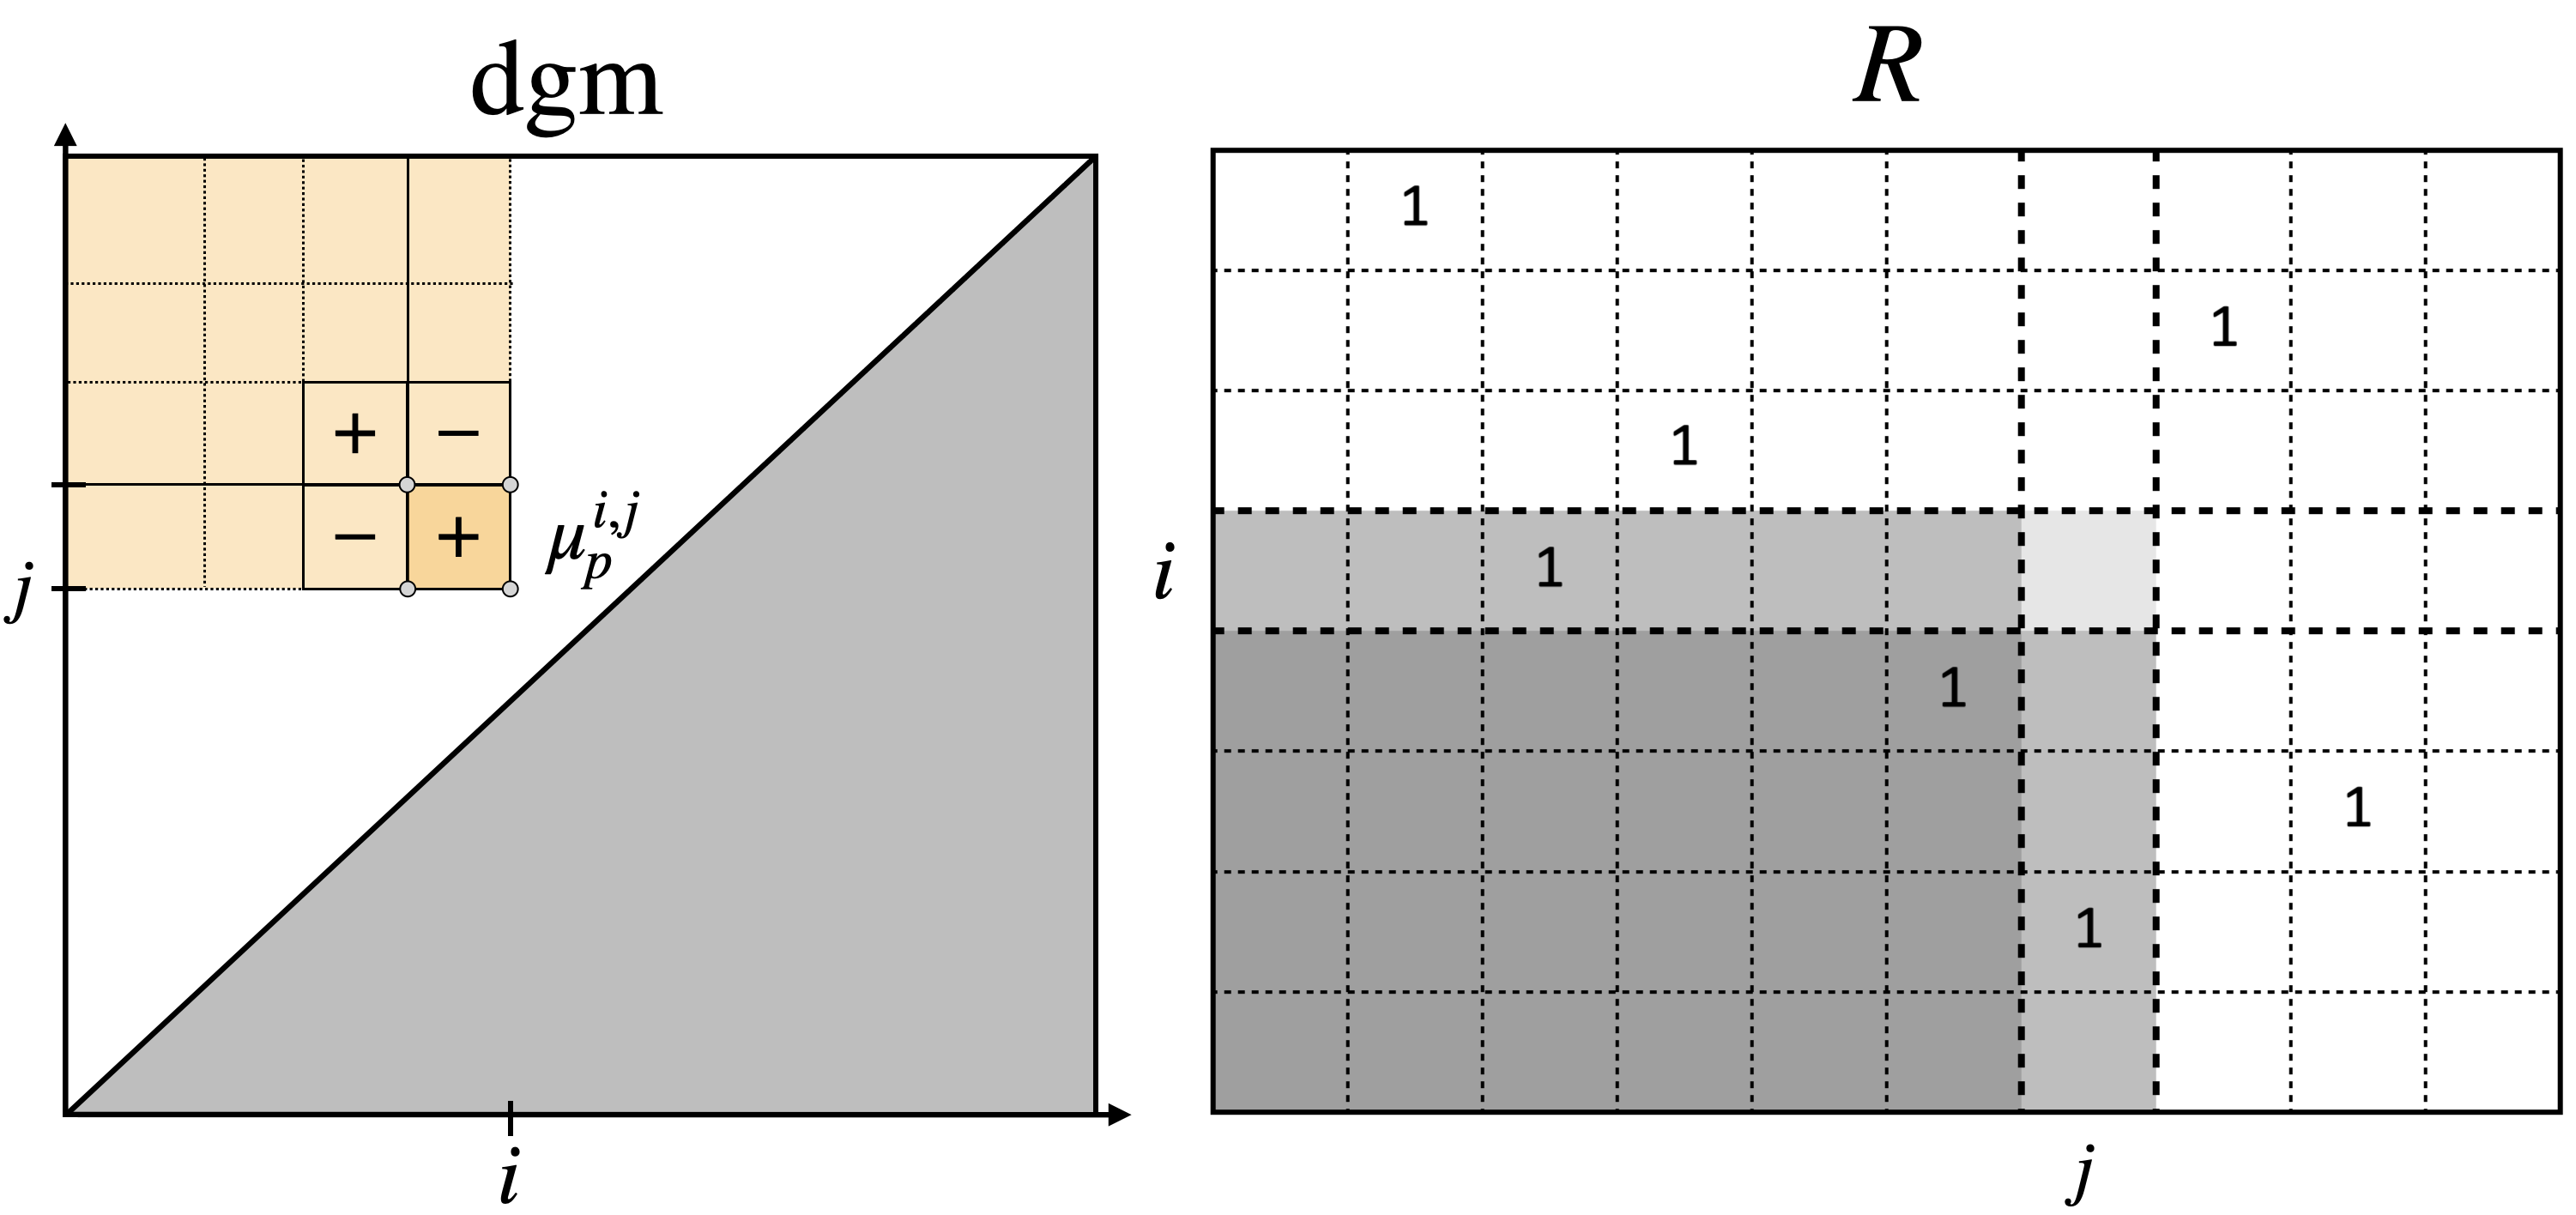
\includegraphics[width=0.45\textwidth]{mult_both}
	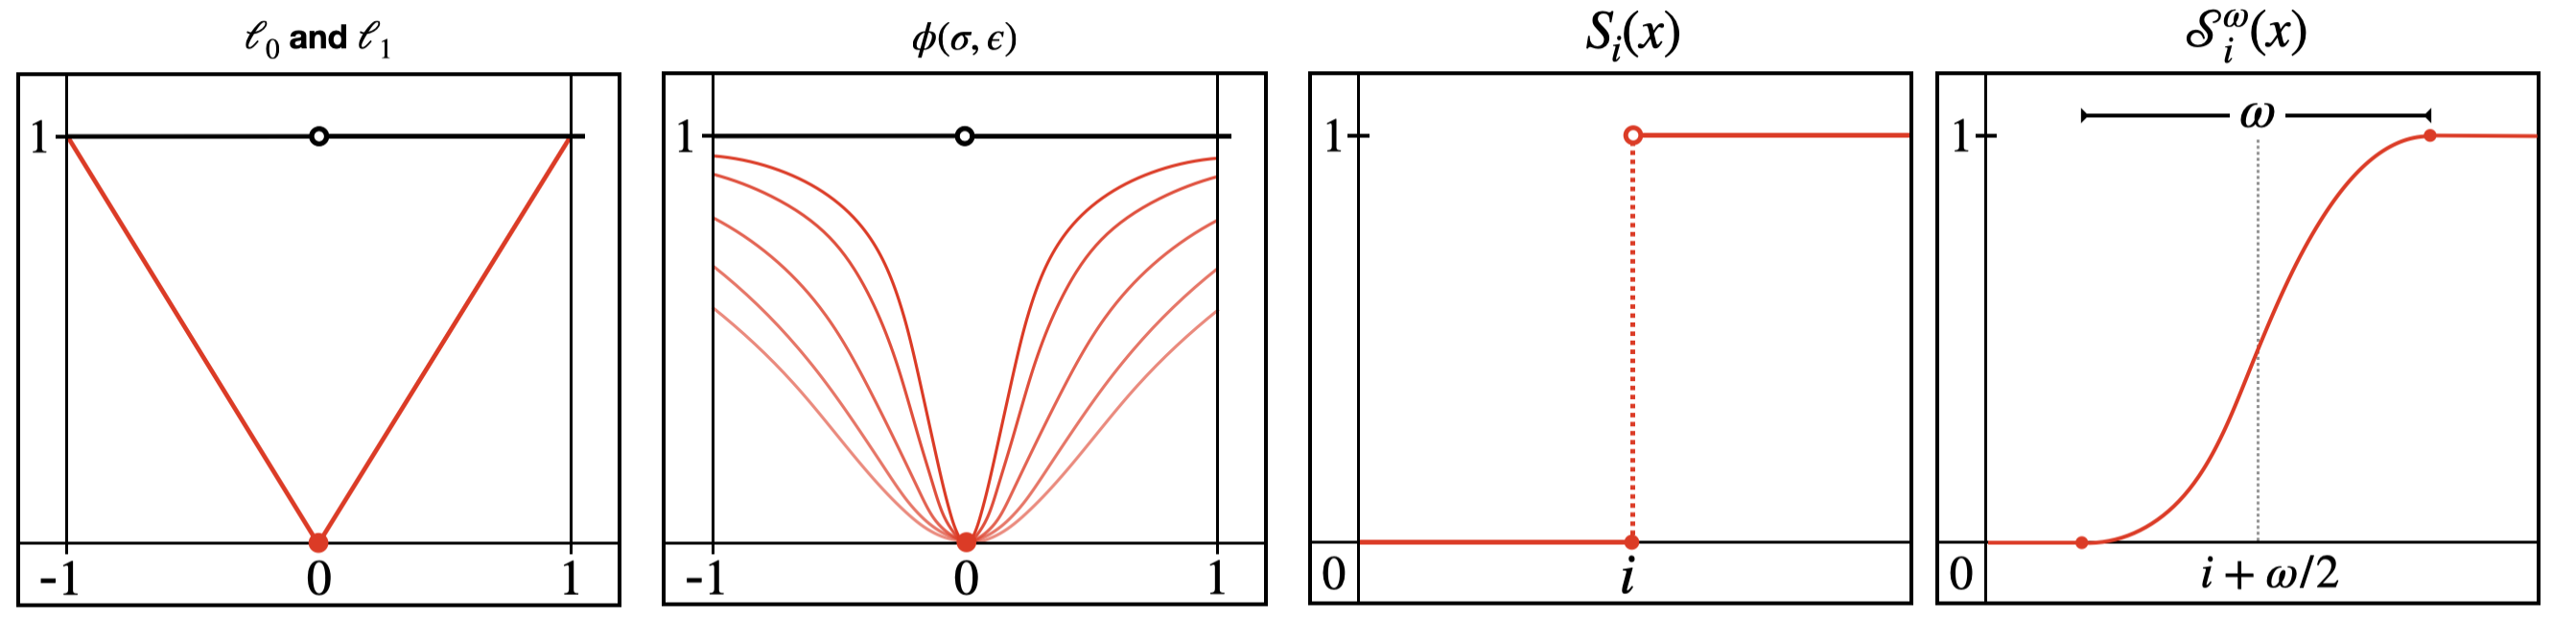
\includegraphics[width=0.90\textwidth]{cont_relax}
	\caption{From left to right: 
	the $\ell_1$ norm (red) forms a convex envelope over the $\ell_0$ (black) pseudo-norm on the interval $[-1, 1]$; 
	$\tilde{\phi}(\cdot, \epsilon)$ at various values of $\epsilon$, with $p(x) = 2x (x^2 + 1)^{-2}$ and $\nu(\epsilon) = \sqrt{\epsilon}$ (red) and at $\epsilon = 0$ (black); 
	the step function $S_i(x)$ from definition~\ref{def:time_boundary_matrix}; 
	the smoothstep relaxation $\mathcal{S}_i^{\omega}$ from~\eqref{eq:smoothstep}.
	}
	\label{fig:smoothstep}
\end{figure}
These are clamped ``S-curve'' functions which interpolate the discontinuous step portion of $S$ along fixed bounds $(a,a+\omega)$, which are given by:  
\begin{equation}\label{eq:smoothstep}
\mathcal{S}_a^{\omega} (x) = \begin{cases}
	0 & x \leq a \\
	S_n\big( \omega^{-1}((a + \omega) - x) \big) & a < x < a + \omega \\
	1 & a + \omega \leq x
\end{cases}
\end{equation} 
%% TODO: Why does the smooth-step call these Hermite polynomials?
where $S_n: [0,1] \to [0,1]$ is a generic $n$-th order polynomial whose coefficients are fixed such that $S_n(0) = 0$ and $S_n(1) = 1$.
%\begin{equation}
%S_n(x)  = a_n x^n + a_{n-1} x^{n-1} + \dots + a_1 x + a_0
%\end{equation} 
These polynomials have found applications computer graphics and machine learning applications~\cite{}. 
Our motivation to use them here is based on the observations shown in Figure~\ref{fig:smoothstep}: by substituting $\mathcal{S}_n^{\omega}$ for the step functions 	in~\eqref{eq:param_boundary_matrix}, we have a version of the parameterized boundary matrix whose entries varies continuously in $\mathcal{H}$ but which retain the same rank as their discontinuous counterparts. 
%We include a short definition:
%\begin{definition}[Continuously Parameterized boundary matrix]\label{def:time_boundary_matrix2}
%Let $K$ denote a fixed simplicial complex and $f: K \times \mathcal{H} \to \mathbb{R}$ a parameterized family of filter functions that varies continuously in $\mathcal{H}$. Assume both respect the same conditions outlined in definition~\ref{def:time_boundary_matrix}. 
%For fixed $(i,j) \in \Delta_{+}$, define the $\mathcal{H}$-\emph{parameterized} $p$\emph{-th boundary matrix} $\tilde{\partial}_p^{i, j}(h)$ \emph{at scale} $(i,j)$ as the matrix whose entries $(k,l)$ satisfy:
%\begin{equation}\label{eq:param_boundary_matrix_cont}
%	\tilde{\partial}_p^{i,j}(h)[k,l] = \begin{cases}
%	% \pm \, S_{i,j}(\sigma_k, \sigma_l) & \text{if } \sigma_k \in \partial_p(\sigma_l) \\
%	\pm \, (\mathcal{S}^\omega_{i} \circ f_h)(\sigma_k)) \cdot (\tilde{\mathcal{S}}^\omega_{j} \circ f_h)(\sigma_l) & \text{if } \sigma_k \in \partial_p(\sigma_l) \\
%	%, \text{ where } \epsilon = f(\sigma_l) \\
%	0 & \text{otherwise}
%\end{cases}
%\end{equation}
%where $\mathcal{S}_{i}^\omega : \mathbb{R} \to \{0, 1\}$ is a \emph{smoothstep} function satisfying~\eqref{eq:smoothstep} and $\tilde{\mathcal{S}}_{i}^\omega = 1 -\mathcal{S}_{i}^\omega$, and $f_h(\sigma) = f(\sigma, h)$.
%\end{definition}
%We summarize the previous 
Moreover, by composing with~\eqref{eq:mu_four} and substituting $\mathrm{rank}(\cdot)$ with $\Phi(\cdot, \epsilon)$ for some $\epsilon > 0$, we obtain $\epsilon$-approximate, continuously-varying multiplicity function. 
\begin{definition}[Continuous Multiplicity]
Let $K$ denote a fixed simplicial complex and $f: K \times \mathcal{H} \to \mathbb{R}$ a parameterized family of filter functions that varies continuously in $\mathcal{H}$. Let $\tilde{\partial}_p$ denote the $\mathcal{H}$-parameterized $p$-th boundary matrix from~\ref{def:time_boundary_matrix} with step functions $S_\ast$ replaced by the smoothstep $\mathcal{S}_\ast^\omega$ from~\eqref{eq:smoothstep}, for some fixed $\omega > 0$. Define the \emph{continuous multiplicity function} over some fixed $R = [i,j] \times [k,l]$ as:
	\begin{equation}\label{eq:mu_cont}
	\hat{\mu}_{p,\epsilon}^R(h) = 
		 \lVert \Phi_\epsilon^h(\tilde{\partial}_{p+1}^{j \+ \delta, k}) \rVert_\ast - 
		 \lVert \Phi_\epsilon^h(\tilde{\partial}_{p+1}^{i \+ \delta, k}) \rVert_\ast -  
		 \lVert \Phi_\epsilon^h(\tilde{\partial}_{p+1}^{j \+ \delta, l}) \rVert_\ast + 
		 \lVert \Phi_\epsilon^h(\tilde{\partial}_{p+1}^{i \+ \delta, l}) \rVert_\ast \numberthis
\end{equation}
where $\Phi_\epsilon^h(\partial) = (\Phi_\epsilon \circ \partial)(h)$ for any $h \in \mathcal{H}$. The formulation of the PBN relaxation is synonymous.
\end{definition}
\noindent Since the sum $f + g$ of two Lipshitz functions $f$ and $g$ is also Lipshitz, it is easy to verify that $\hat{\mu}_p^R$ is Lipshitz continuous by combining the smoothness of $\mathcal{S}_\ast^\omega$ with the global Lipshitz continuity of~\eqref{def:cont_rank}. 
%\begin{corollary}
%	For every matrix $$ any $\epsilon > 0$, the approximations $\beta_p$ and $\tilde{\mu}_p^\ast$ vary continuously in $\mathcal{H}$. Moreover, there exists some $\bar{\epsilon} > 0$ such that: 
%	$$ \lfloor \tilde{\beta}_p^{\ast}(K) \rfloor = $$
%\end{corollary}
%These approximations are also "betti-like". 

%% REVISIT LAPLACIAN!



% The stability of the spectral relaxation proposed in~\eqref{} lends some stability the computation of the Betti and Multiplicity computations we have discussed in parameterized setting. 

\section{Parameterized setting \& Perturbation theory}
If $f$ is a real-valued filter function that various smoothly in $\mathcal{H}$, one would expect the spectra of the constitutive terms in $\beta_p^\ast$ and $\mu_p^\ast$ to also vary smoothly as functions of $\mathcal{H}$.
Indeed, since Laplacian matrices are normal matrices, we expect their spectra to be quite stable under perturbations~\cite{}. 
%Moreover,

% The spectrum of Normal matrices are stable: if A is normal and is perturbed by a perturbation w/ norm at most \epsilon, then the spectrum moves by at most \epsilon. And Laplacian matrices are normal matrices
% https://terrytao.wordpress.com/2008/10/28/when-are-eigenvalues-stable/
%In what follows, we fix $p \geq 0$ and use $L_{(h)}^{i,j}$ to denote the $p$-th up Laplacian at time $h \in \mathcal{H}$.
%Let $\hat{\partial}_h$

% Rayleigh-Ritz discussion
\textbf{Rayleigh Ritz values}
Though the Lanczos iterations may be used to obtain the full tridiagonalization $A = Q T Q^T$,  intermediate spectral information is readily available in $T_j$, for $j < \mathrm{rank}(A)$.
% Even before an $A$-invariant subspace is obtained, 
%If $T_j$ represents projection of $A$ onto the $j$-th Krylov subspace $\mathcal{K}_j(A, q_1)$, 
Diagonalizing $T_j = Y \Theta Y^T$ yields value/vector pairs $\{  (\theta_1^{(j)}, y_1^{(j)}), \dots, (\theta_j^{(j)}, y_j^{(j)}) \}$ satisfying $w^T (Ay - \theta y) = 0$ for all $w \in \mathcal{K}_j(A, q_1)$, called \emph{Ritz pairs}. The values $\theta$ are called \emph{Ritz values} and their associated vectors $v = Q y$ in the range of $Q$ are called \emph{Ritz vectors}.
From the Ritz perspective, the Lanczos iteration implicitly maintains two orthonormal basis for $K_j(A, q_1)$---a Lanczos basis $Q$ and the Ritz basis $Y$:
$$ A = Q T Q^T = Q Y \Theta Y^T Q^T \Longleftrightarrow A Q Y = Q Y \Theta $$
In principle, the Lanczos basis $\{q_i\}_{i=1}^j$ changes each iteration, while the Ritz basis $\{ Q y_i^{(j)} \}_{i=1}^{j}$ changes after each subspace projection. The way in which the Ritz values approach the spectrum of $A$ is well-studied~\cite{}, as they are known to be Rayleigh-Ritz approximations of $A$'s eigenpairs $\Lambda(A) = \{  (\lambda_1, v_1), \dots, (\lambda_j, v_j) \}$, and they are collectively known to be optimal in the sense that $T_k = B$ is the matrix that minimizes $\lVert A Q_k - Q_k B \rVert_2$ over the space of all $k \times k$ matrices. 
Moreover, Ritz values contain intrinsic information of the distance between $\Lambda(T_j)$ and $\Lambda(A)$. To see this, note that: 
\begin{equation}
	\lVert A v_i^{(j)} - v_i^{(j)} \theta_i^{(j)} \rVert = \beta_i^{(j)} = \beta_{j+1} \cdot \lvert \langle e_j, y_i^{(j)} \rangle   \rvert 
\end{equation}
Thus, we need not necessarily keep the Lanczos vectors $Q$ in memory to monitor how close the spectra of the $T_j$'s approximate $\Lambda(A)$. In fact, it is known that the Ritz values $\{ \theta_1^{(1)}, \theta_1^{(2)}, \dots, \theta_1^{(j)} \}$ of $T_j$ satisfy: 
 \begin{equation}
 	\lvert \lambda - \theta_i^{(j)} \rvert \leq \big ( \beta_i^{(j)} \big )^2 / \big( \min_\mu \; \lvert \mu - \theta_i^{(j)} \rvert \big ) 
 \end{equation}
The full convergence of the Ritz values to the eigenvalues of $A$ is known to converge at a rate that depends on the ratio between $\lambda_1/\lambda_n$. A full analysis is done in terms of Chebychev Polyonomials in~\cite{golub2013matrix}. In practice, it has been observed that the Lanczos iteration converges super-linearly towards the extremal eigenvalues of the spectrum, whereas for interior eigenvalues one typically must apply a shifting scheme.

\subsection{(1-$\epsilon$) Approximations}
Note that when $\nu(\epsilon) = \sqrt{\epsilon}$ and $p(x) = 2x (x^2 + 1)^{-2}$, Equation~\eqref{def:cont_rank} reduces to: 
\begin{equation*}
	\lVert \Phi_\epsilon(X) \rVert_\ast = \sum\limits_{i = 1}^n \frac{\sigma_i(X)^2}{\sigma_i(X)^2 + \epsilon} = \mathrm{Tr}\left[X^T (X X^T + \epsilon \, I_n) X \right] 
\end{equation*}
which is the generic rank approximation studied by~\cite{}. Moreover, by the cyclic property of the trace operator, since $X = \partial_1$ here and $L = \partial_1 \partial_1^T = [l_1, l_2, \dots, l_n]$ we have: 
\begin{equation*}
	\lVert \Phi_\epsilon(X) \rVert_\ast = \mathrm{Tr}[(L + \epsilon I_n)^{-1} L] = \sum\limits_{i=1}^n (L_\epsilon^{-1} l_i)_i
\end{equation*}
Thus we may solve this problem by solving $n$ sparse linear systems of that take the form $Ax = b$, where here $A$ is a Laplacian matrix with an $\epsilon \cdot I_n$ addition to it's diagonal. 
From this expression, it's clear that $\epsilon$ not only plays the role of an accuracy parameter, but as a smoothing parameter. Indeed, define the condition number

Small condition numbers often improve the convergence of iterative solvers and improve stability of spectrum with respect to perturbations in the entries of the matrix. 
$\kappa(M^{-1} A)$

% the desired effect in applying a preconditioner is to make the quadratic form of the preconditioned operator {\displaystyle P^{-1}A}P^{{-1}}A with respect to the {\displaystyle P}P-based scalar product to be nearly spherical.
$$
M^{-1} A x = M^{-1}b 
$$
where $M$ is symmetric positive definite. 
\begin{equation}
	\min_{x \perp \mathbf{1} } \frac{1}{2} x^T (L + \epsilon I_n) x - b^T x
\end{equation}
Since this nonsingular, positive definite, strictly diagonally dominant matrix, thus we may apply the famous Conjugate Gradient (CG) algorithm to solve such a system. It's well known that CG converges to the solution of $A x = b$ in exactly $O(n)$ iterations (and often much earlier), of which each iteration requires one $O(m)$ matrix-vector product, implying a runtime of $O(mn^2)$ (compare with...).  
%http://www.cs.yale.edu/homes/spielman/561/2009/lect16-09.pdf
Moreover, and since this is a Laplacian matrix, the wealth of tools developed for said matrices may also be used.
In particular, ~\cite{} showed that \emph{low-stretch spanning trees} act as good preconditioners to accelerate Laplacian solvers, wherein it's been shown that the preconditioned Conjugate Gradient (PCG) requires as most $O(\sqrt{m} \log n)$ iterations, each of which requires one matrix-vector product using $L_G$ and in $O(m^{1/3} \log n \, \mathrm{ln} 1/\epsilon)$ iterations. 
This was later improved by, who showed that one can solve Laplacian systems effectively in $O(m \log^{O(1)} n)$ time, giving a bound of $O(r m \log^{O(1)} n)$ time to obtain.... 

Of course, if one wants to compute either of the counting invariants in... exactly for $p = 0$, of course, the fastest algorithm is to reduce the problem to the well-known elder-rule problem, which takes $O(m \log m + m \alpha(n))$ time for a general filtration. It is unlikely that we may beat this bound, either in theory or in practice, for $p = 0$.
However, the fastest known algorithm for computing the full persistence diagram for $p \geq 1$ is $O()$, which is quite a jump in complexity; there is no generalization of disjoint-set algorithm for the case where $p \geq 1$. 
Moreover, these direct methods tend to be memory bound operations, pushing researchers who want to compute these diagrams in practice to focus on ways of reducing the memory usage, such as using $\mathbb{Z}_2$ field coefficients. 
In contrast, the means by which we compute these invariants scales quite well with larger $p$, it produces a stronger invariant, and is far more reaching to other areas of mathematics. 


\newpage

\newpage

\section{Applications}\label{sec:applications}

% TODO: See seminar "Persistent Homology with Random Graph Laplacians"

% --- APPLICATION 1: Fast Dgm computation ---
%\subsection*{Complexity}
% \subfile{rank_complexity} % include numerical rank definition



% --- APPLICATION 2: Continuous Persistent Betti Curves (PBCs) as Shape Signatures --- 
% Benefits of rank(A) \approx < nuclear norm of A >
%\subsection*{Application: Relaxation}
%\subfile{spectral_relaxation}
% TODO: ask Jose + Luis how to describe this better
As topological invariants, Betti numbers are invariant under homeomorphisms: any pair of filtrations $(K, f)$ and $(K', f')$ that are homotopy equivalent have identical homology classes and thus isomorphic persistence diagrams. 
This invariance can be a useful thing at the level of homology, as non-homeomorphic spaces can sometimes be differentiated by inspecting differences between their corresponding homology classes. 
However, invariance under homeomorphisms can at times discard geometric information that may be useful for differentiating objects.
For example, consider creating a classifier for the alphabet of English characters in the font shown below:
\vspace{0.5em}
\\
\vspace{0.5em}
\begin{ttfamily}
	\fontfamily{lmss}\selectfont \bfseries
	\hfill A B C D E F G H I J K L M N O P Q R S T U V W X Y Z \hfill 
\end{ttfamily}

\noindent If one were to triangulate images of each of the letters shown above and compute their Betti numbers, one would find just three homology classes: one class for those letters that have two holes (B), one class of letters that have one hole (A, D, O, P, Q, and R), and one class for the rest of the letters, which collapse to points. It would be beneficial to have an invariant that was sensitive to the geometries between shapes, but also also stable in some sense.

\newpage

% --- APPLICATION 3: Directional transforms ---- 
\subsection*{Directional Transform}
The canonical interpretation of the information displayed by a persistence diagram is that is summarizes the persistence of the sublevel sets of filtered space. Given a filtration pair $(\, K, f \, )$ where $K$ is a finite simplicial complex and $f : K \to \mathbb{R}$ is a real-valued function, the sublevel sets $\lvert K \rvert_i=f^{-1}(-\infty, i]$ deformation retract to... % say more about stars, homotopy equivalence
% simplexwise-linear function
% http://www.csun.edu/~ctoth/Handbook/chap24.pdf
If $K$ is embedded in $\mathbb{R}^d$, then geometrically $f$ takes on the interpretation of a `height' function whose range yields the `height' of every simplex in $K$. 
%Obviously, this notion of height depends on the embedding of $K$: viewing $K$ (and thus, $X$) from different `directions' induces potentially distinct sublevel sets, 

%Given a simplicial complex $K$ embedded in $\mathbb{R}^d$, 
Let $X \subset \mathbb{R}^d$ denote a data set which can be written as a finite simplicial complex $K$ whose simplices are PL-embedded in $\mathbb{R}^d$. Given this setting,  define the \emph{directional transform} (DT) of $K$ as follows:
\begin{align*}\label{eq:pht}
	\mathrm{DT}(K): S^{d-1} &\to  K \times C(K, \mathbb{R}) \\
	v &\mapsto (K_\bullet, f_v)
\end{align*}
where we write $(K_\bullet, f)$ to indicate the filtration on $K$ induced by $f_v$ for all $\alpha \in \mathbb{R}$, i.e.: 
\begin{equation}
	K_\bullet = K(v)_\alpha = \{\, x \in X \mid \langle x, v \rangle \leq \alpha  \,\} %_{\alpha = -\infty}^{\infty}
\end{equation}
Conceptually, we think of DT as an $S^{d-1}$-parameterized family of filtrations. 

% Conceptually, the $p$-th dimensional persistence diagram $\mathrm{dgm}_p(K, v)$ summaries how the topology of the filtration $K(v)$ changes in the direction of  $v$. Similarly, the PHT summarizes how the topology of $K$ changes in \emph{all} directions

The Persistent Homology Transform (PHT) is a shape statistic that establishes a fundamental connection between the topological information summarized by $K$'s PH groups and the geometry of its associated embedding. Given a complex $K$ built from $X$, it is defined as: 
\begin{align*}\label{eq:pht}
	\mathrm{PHT}(K): S^{d-1} &\to \mathcal{D}^d \\
	v &\mapsto \left( \, \mathrm{dgm}_0(K, v), \mathrm{dgm}_1(K, v), \dots, \mathrm{dgm}_{d-1}(K, v) \, \right)\numberthis
\end{align*}
where $\mathcal{D}$ denotes the space of $p$-dimensional persistence diagrams, for all $p = 0, \dots, d-1$ and $S^{d-1}$ the unit $d-1$ sphere. The stability of persistence diagrams ensures that the map $v \mapsto \mathrm{dgm}_p(K, v)$ is Lipschitz with respect to the bottleneck distance metric $d_B(\cdot, \cdot)$ whenever $K$ is a finite simplicial complex. 
Thus, the PHT may be thought of as an element in $C(S^{d-1}, \mathcal{D}^d)$: . 

%thus the PHT may be thought of naturally as a parameterized family of diagrams.

The primary result of~\cite{} is that the PHT is injective on the space of subsets of $R^d$ that can be written as finite simplicial complexes\footnote{Implicit in the injectivity statement of the PHT is that, given a subset $X \subset \mathbb{R}^d$ which may be written as finite simplicial complex $K$, the restriction $f: X \to \mathbb{R}$ to any simplex in $K$ must is linear.}, which we denote as $\mathcal{K}_d$. 
Equivalently, $\mathcal{K}_d$ decomposes space of all pairs $(K, f)$ under the equivalence $(K, f) \sim (K,f')$ when $f(K) = f'(K)$.

%Like the directional transform, the PHT is essentially the ompositon of the DT with PH: PHT= PH \circ DT. 
% One of the constructing metrics capable of differentiating non-diffeomorphic shapes.
 

\appendix
\section{Appendix}
\subsection{Finite-precision arithmetic}\label{subsec:rounding} 
It is well established in the literature that the Lanczos iteration, as given in its original form, it effectively useless in practice due to significant rounding and cancellation errors. Such errors manifest as loss of orthogonality between the computed Lanczos vectors, which drastically affects the convergence of the method. 
At first glance, this seems to be a simple numerical issue, however the analysis from Parlett~\cite{parlett1994we} showed, loss of orthogonality is not merely the result of gradual accumulation of roundoff error---it is in fact is intricately connected to the convergence behavior of Lanczos iteration. 
One obvious remedy to this is to reorthogonalize the current Lanczos vectors $\{q_{j-1}, q_{j}, q_{j+1}\}$ against all previous vectors using Householder matrices~\cite{golub2013matrix}---a the \emph{complete reorthogonalization} scheme. This process guarantees orthogonality to working precision, but incurs a cost of $O(jn)$ for each Lanczos step, effectively placing the iteration back into the cubic time and quadratic memory regimes the direct methods exhibit. 
A variety of orthogonality enforcement schemes have been introduced over years, including implicit restart schemes, selective reorthogonalization, thick restarts, block methods, and so on; see~\cite{} for an overview.  

\subsection{Laplacian Interpretation}
In what follows we make a connection between boundary matrices and the graph Laplacian to illustrate how the Laplacian captures the ``connectivity'' aspects of the underlying simplicial complex. 
 \begin{example}[Adapted from~\cite{newman2001laplacian}]\label{ex:laplacian}
Suppose the vertices of $G$ are ordered and labeled from $1$ to $n$ arbitrarily such that, given any subset $X \subseteq V$, we may define column vector $x = (\, x_i\, )$ whose components $x_i = 1$ indicate $i \in X$ and $x_i = 0$ otherwise. Given such a set $X \subseteq V$, let $X' = V \setminus X$ denote its complement set. By $L$'s definition, we have:
\begin{align*}
	(Lx)_i > 0 &\Longleftrightarrow i \in X \text{ and } \lvert c_i(X) \rvert = (Lx)_i  \\
	(Lx)_i < 0 &\Longleftrightarrow i \in X' \text{ and } \lvert c_i(X') \rvert = \lvert (Lx)_i \rvert \\
	(Lx)_i = 0 &\Longleftrightarrow i \in X \cup X' \text{ and } c_i(X) = \emptyset
\end{align*}
where $c_v(X) = \{ (v,w) \in E \mid v \in X \text{ and } w \in V \setminus X \}$ denotes the \emph{cutset}  of $X$ restricted to $v$, i.e. the set of edges having as one endpoint $v \in X$ and another endpoint outside of $X$.
\end{example}
\noindent In other words, example~\ref{ex:laplacian} demonstrates that $L$ captures exactly how $X$ is connected to the rest of $G$. Notice that if $X  = V$, then $Lx = 0$ and thus $0$ must be an eigenvalue of $L$ with an eigenvector pair $\mathbf{1}$. Like the adjacency matrix, the interpretation of the matrix-vector product has a natural extension to powers of $L$, wherein just as entries in $A^k$ model paths, entries in $L^k$ are seen to model boundaries~\cite{newman2001laplacian}.

\subsection*{Applications}
We include a few examples of potential application areas of work. Namely, we show a few promising examples of ``parameterized settings'' that may naturally benefit from our efforts here.
\\
\\ 
\textbf{Dynamic Metric Spaces:} Consider an $\mathbb{R}$-parameterized metric space $\delta_X = ( X, d_X(\cdot) )$ where $X$ is a finite set and $d_X(\cdot): \mathbb{R} \times X \times X \to \mathbb{R}_{+}$, satisfying: 
\begin{enumerate}
	\item For every $t \in \mathbb{R}, \delta_X(t) = (X, d_X(t))$ is a pseudo-metric space\footnote{This is required so that if one can distinguish the two distinct points $x, x' \in X$ incase $d_X(t)(x, x') = 0$ at some $t \in \mathbb{R}$. } 
	\item For fixed $x, x' \in X$, $d_X(\cdot)(x, x'): \mathbb{R} \to \mathbb{R}_{+}$ is continuous.
\end{enumerate}
When the parameter $t \in \mathbb{R}$ is interpreted as \emph{time}, the above yields a natural characterization of a ``time-varying'' metric space. More generally, we refer to an $\mathbb{R}^h$-parameterized metric space as \emph{dynamic metric space}(DMS). 
Such space have been studied more in-depth~\cite{} and have been shown...


%Let $\delta_\mathcal{X}$ denote an $\mathrm{T}$-parameterized metric space $\delta_\mathcal{X}(\cdot) = ( X, d_X(\cdot) )$, where $d_X: \mathrm{T} \times X \times X \to \mathbb{R}_+$ is called a \emph{time-varying metric}  and $X$ is a finite set with fixed cardinality $\lvert X \rvert = n$. $\delta_X$ as called a \emph{dynamic metric space} (DMS) iff $d_X(\cdot)(x, x')$ is continuous for every pair $x, x' \in X$ and $\delta_\mathcal{X}(t) = (X, d_X(t))$ is a pseudo-metric space for every $t \in \mathrm{T}$. 
%For a fixed $t \in \mathrm{T}$, the Rips complex at scale $\epsilon \in \mathbb{R}$ is the abstract simplicial complex given by 
%\begin{equation}
%	\mathrm{Rips_{\epsilon}}(\delta_\mathcal{X}(t)) := \{ \sigma \subset X : d_X(t)(x, x') \leq \epsilon \text{ for all } x, x' \in \sigma \}
%\end{equation}
%\noindent As before, the family of Rips complexes for varying $\epsilon > 0$ yields a filtration whose inclusion maps induce linear maps at the level of homology. The time-varying counterpart is analogous.  
%In this context, we write the $p$-th persistent Betti number with respect to fixed values $i,j \in I$ as a function of $t \in \mathrm{T}$: 
%\begin{equation}
%\beta_{p}^{i,j}(t) = \left(\mathrm{dim} \circ \mathrm{H}_p^{i,j} \circ \mathrm{Rips} \circ \delta_\mathcal{X} \right)(t)
%\end{equation}


\subsection{Proofs}
\subsubsection*{Proof of Lemma 1}
\begin{proof}
	The Pairing Uniqueness Lemma~\cite{dey2022computational} asserts that if $R = \partial V$ is a decomposition of the total $m \times m$ boundary matrix $\partial$, then for any $1 \leq i < j \leq m$ we have $\mathrm{low}_R[j] = i$ if and only if $r_\partial(i,j) = 1$. 
	As a result, for $1 \leq i < j \leq m$, we have:
\begin{equation}
	\mathrm{low}_R[j] = i \iff r_R(i,j) \neq 0 \iff r_\partial(i,j) \neq 0
\end{equation} 
Extending this result to equation~\eqref{eq:lower_left_rank} can be seen by observing that in the decomposition, $R = \partial V$, the matrix $V$ is full-rank and obtained from the identity matrix $I$ via a sequence of rank-preserving (elementary) left-to-right column additions.  
\end{proof}

\subsubsection*{Proof of Proposition 1}
\begin{proof}
We first need to show that $\beta_p^{i,j}$ can be expressed as a sum of rank functions. Note that by the rank-nullity theorem, so we may rewrite~\eqref{eq:pbn} as:
%$$ \beta_p^{i,j} = \mathrm{dim} \left( Z_p(K_i) \right) - \mathrm{dim}\left( Z_p(K_i) \cap B_p(K_j) \right ) $$
$$ \beta_p^{i,j} = \mathrm{dim} \left( C_p(K_i) \right) - \mathrm{dim} \left( B_{p-1}(K_i) \right) - \mathrm{dim}\left( Z_p(K_i) \cap B_p(K_j) \right ) $$
The dimensions of groups $C_p(K_i)$ and $B_p(K_i)$ are given directly by the ranks of diagonal and boundary matrices, yielding:  
$$
	\beta_p^{i,j} = \mathrm{rank}(I_p^{1, i}) - \mathrm{rank}(\partial_p^{1,i}) - \mathrm{dim}\left( Z_p(K_i) \cap B_p(K_j) \right )
$$
To express the intersection term, note that we need to find a way to express the number of $p$-cycles born at or before index $i$ that became boundaries before index $j$. 
Observe that the non-zero columns of $R_{p \+ 1}$ with index at most $j$ span $B_p(K_j)$, i.e $\{ \, \mathrm{col}_{R_{p\texttt{+}1}[k] } \neq 0 \mid \, k \in [j] \,\} \in \mathrm{Im}(\partial_{p+1}^{1,j})$. Now, since the low entries of the non-zero columns of $R_{p \+ 1}$ are unique, we have:
\begin{equation}\label{eq:s1}
	\mathrm{dim}(Z_p(K_i) \cap B_p(K_i)) = \lvert \Gamma_p^{i,j} \rvert
\end{equation}
where $\Gamma_p^{i,j}  = \{ \, \mathrm{col}_{R_{p\texttt{+}1}[k] } \neq 0 \mid \, k \in [j], \, 1 \leq \mathrm{low}_{R_{p\texttt{+}1}}[k] \leq i \,\}$. Consider the complementary matrix $\bar{\Gamma}_p^{i,j}$, given by the non-zero columns of $R_{p \+ 1}$ with index at most $j$ that are not in $\Gamma_p^{i,j}$, i.e. the columns satisfying $\mathrm{low}_{R_{p\texttt{+}1}}[k] > i$. Combining rank-nullity with the observation above, we have: 
\begin{equation}\label{eq:s2}
	 \lvert \bar{\Gamma}_p^{i,j} \rvert = \mathrm{dim}(B_p(K_j)) - \lvert \Gamma_p^{i,j} \rvert = \mathrm{rank}(R_{p\+1}^{i\+1,j})
\end{equation}
Combining equations~\eqref{eq:s1} and~\eqref{eq:s2} yields:
\begin{equation}\label{eq:s3}
	\mathrm{dim}(Z_p(K_i) \cap B_p(K_j))  = \lvert \Gamma_p^{i,j}  \rvert 
	= \mathrm{dim}(B_p(K_j)) -  \lvert \bar{\Gamma}_p^{i,j}  \rvert 
	= \mathrm{rank}(R_{p\+1}^{1, j}) - \mathrm{rank}(R_{p\+1}^{i\+1,j})
\end{equation}
Observing the final matrices in~\eqref{eq:s3} are \emph{lower-left} submatrices of $R_{p\+1}$, the final expression~\eqref{eq:betti_four} follows by applying Lemma~\ref{lemma:rank} repeatedly. 
\end{proof}

\subsubsection*{Proof of boundary matrix properties}
\begin{proof}
First, consider property (1). For any $t \in T$, applying the boundary operator $\partial_p$ to $K_t = \mathrm{Rips}_\epsilon(\delta_{\mathcal{X}}(t))$ with non-zero entries satisfying~\eqref{eq:matrix_pchain} by definition yields a matrix $\partial_p$ satisfying $\mathrm{rank}(\partial_p) = \mathrm{dim}(\mathrm{B}_{p-1}(K_t))$. In contrast, definition~\eqref{def:time_boundary_matrix} always produces $p$-boundary matrices of $\Delta_n$; however, notice that the only entries which are non-zero are precisely those whose simplices $\sigma$ that satisfy $\mathrm{diam}(\sigma) < \epsilon$. Thus, $\mathrm{rank}(\partial_p^t) = \mathrm{dim}(\mathrm{B}_{p-1}(K_t))$ for all $t \in T$. 
$<$ (show proof of (2))$>$
Property (3) follows from the construction of $\partial_p$ and from the inequality $\lVert A \rVert_2 \leq \sqrt{m} \lVert A \rVert_1$ for an $n \times m$ matrix $A$, as $\lVert \partial_p^t \rVert_1 \leq (p+1) \, \epsilon$ for all $t \in T$.

	% Assume that $\delta_{\mathcal{X}}$ is $C$-Lipshitz. Then $d_X(t)(x, x') \leq C d_X(t')(x, x')$ for all $x, x' \in X$, then observe $\partial_p^\ast$. 
\end{proof}



%\subsection*{Rank relaxation}
%A common approach in the literature to optimize quantities involving $\mathrm{rank}(A)$ for some $m \times n$ matrix $A$ is to consider optimizing its \emph{nuclear norm} $\lVert A \rVert_\ast = \mathrm{tr}(\sqrt{A^T A}) = \sum_{i=1}^r \lvert \sigma_i \rvert$, where $\sigma_i$ denotes the $i$th singular value of $A$ and $r=\mathrm{rank}(A)$. One of the primary motivations for this substitution is that the nuclear norm is a convex envelope of the rank function over the set: 
%$$
%S := \{ A \in \mathbb{R}^{n \times m} \mid \lVert A \rVert_2 \leq m \}
%$$
%That is, for an appropriate $m > 0$, the function $A \mapsto \frac{1}{m}\lVert A \rVert_\ast$ is a lower convex envelope of the rank function over $S$. The nuclear norm also admits a subdifferential... thus, we may consider replacing~\eqref{} with: 
%\begin{align}\label{eq:betti_four_nuc}
%	\beta_p^{i,j}(t) &= \lvert \partial_{p,t}^{1,i} \rvert -
%	m_1\inv \lVert \partial_{p,t}^{1,i} \rVert_\ast - 
%	m_2\inv \lVert \partial_{\bar{p},t}^{1,j}\rVert_\ast - 
%	m_3\inv \lVert\partial_{\bar{p},t}^{\bar{i},j}\rVert_\ast 
%\end{align}
%where $\bar{c} = c + 1$. Now, if $t \mapsto \partial_p^\ast(t)$ is a non-decreasing, convex function in $t$, then the composition ... is convex, as each of the individual terms are convex. Moreover, we have...
%
%$<$ Insert proof about this relaxation always lower-bounding $\beta$ $>$

%\subsection*{Computation}
%In this section, we discuss the computation of suitable bases for the subspaces $Z_p(X_\ast)$, $B_p(K_\ast)$, and $Z_p(X_\ast) \cap B_p(X_\ast)$. In particular, we address two cases: the \emph{dense} case, wherein the aforementioned bases are represented densely in memory, and the \emph{sparse} case, which uses the structure of a particular decomposition of the boundary matrices to derive bases whose size in memory inherits the sparsity pattern of the decomposition.
%\\
%\\
%\textbf{Sparse case:} We require an appropriate choice of bases for the groups $B_{p-1}(K_\ast)$ and $Z_p(X_\ast) \cap B_p(X_\ast)$. 
%For some fixed $t \in T$, let $R_p = \partial_p V_p$ denote the decomposition discussed above, and let $b, d \in \mathbb{R}_+$ be fixed constants satisfying $b \leq d$. Since the boundary group $B_{p-1}(K_b)$ lies in the image of the $\partial_{p}$, it can be shown that a basis for the boundary group $B_{p-1}(K_\ast)$ is given by: 
%\begin{flalign}
%	&& M_p^b = \{ \, \mathrm{col}_{R_{p+1}}(j) \neq 0 \mid j \leq b \, \}  && span()
%\end{flalign}
%Moreover, since $B_{p-1}(K_b) = \mathrm{Im}(\partial_p^b)$, we have $\mathrm{span}(M_p^b) = B_{p-1}(K_b)$ and thus $\mathrm{rank}(M_p^b) = \mathrm{rank}(\partial_p^b)$. Indeed, it can be shown that every lower-left submatrix of $\partial_p^\ast$ satisfies $\mathrm{rank}(\partial_p^\ast) = \mathrm{rank}(R_p^\ast)$. Thus, although $M_p^b$ does provide a minimal basis for the boundary group $B_{p-1}(K_b)$, it is unneeded here. 
%
%A suitable basis for the cycle group can also be read off from the reduced decomposition directly as well. Indeed, let $R_p = \partial_p V_p$ as before. Then the cycle group is spanned by linear combinations of columns of $V_p$: 
%\begin{equation}
%	Z_p^b = \{ \, \mathrm{col}_{V_p}(j) \mid \mathrm{col}_{R_{p}}(j) = 0, j \leq b \, \}	
%\end{equation}
%The formulation of a basis spanning $Z_p(K_i) \cap B_p(K_j)$ is more subtle, as we can no longer use the  fact that every lower-left submatrix of $R_p$ has the same rank as the same lower-left submatrix of $\partial_p$. 
%Nonetheless, a basis for this group can be obtained by reading off specific columns from $R_p$: 
%\begin{equation}
%	M_p^{b, d} := \{\, \mathrm{col}_{R_{p+1}}(k) \neq 0 \mid 1 \leq k \leq d \text{ and } 1 \leq \mathrm{low}_\mathrm{R_{p+1}}(k) \leq b \, \}
%\end{equation}
%%\begin{flalign}
%%	(\, Z_p(K_i) \cap B_p(K_j) \, ) && M_p^{b, d} := \{\, \mathrm{col}_{R_p}(k) \mid 1 \leq k \leq d \text{ and } 1 \leq \mathrm{low}_\mathrm{R_p}(k) \leq b \, \} &&
%%\end{flalign}
%One can show that $M_b^d$ does indeed span $Z_p(X_\ast) \cap B_p(X_\ast)$ by using the fact that the non-zero columns of $R_p$ with indices at most at most $d$ form a basis for $B_p(K_d)$, and that each low-row index for every non-zero is unique. 
%%The issue here is that 
%\\
%\\
%\noindent
%\textbf{Dense case:} 
%In general, persistent homology groups and its various factor groups are well-defined and computable with the reduction algorithm with coefficients chosen over any ring. By applying operations with respect to a field $\mathbb{F}$, both the various group structures $Z_p(K_\bullet) \subseteq B_p(K_\bullet)  \subseteq C_p(K_\bullet) $ and their induced quotient groups $H_p(K_\bullet)$ are vector spaces; thus, the computation of suitable bases can be approached from a purely linear algebraic perspective.
%In particular, by fixing $\mathbb{F} = \mathbb{R}$, we inherit not only many useful tools for obtaining suitable bases for these groups, but also access to their corresponding optimized implementations as well. 
%
%Consider the $p$-th boundary operator $\partial_p^\ast : C_p(K_\ast) \to C_{p-1}(K_\ast)$ whose matrix realization with respect to some choice of simplex ordering $\{\sigma_i\}_{1 \leq i \leq m}$ we also denote with $\partial_p$. By definition, the boundary group $B_p(K_\ast)$ is given by the image $\mathrm{Im}(\partial_{p+1}^\ast) = B_p(K_\ast)$, thus one may basis for $B_p(K_\ast)$ by computing the considering the first $r > 0$  columns of the reduced SVD: 
%\begin{equation}
%	M_p^\ast = [\, u_1 \mid u_2 \mid \dots \mid u_r \, ] = \{ \,  \, \}
%\end{equation}
%
%
%\subsection{Old}
%
%We consider the problem of maximizing the $p$-th \emph{persistent} Betti number $\beta^{i,j}_p$ over some set $T \subseteq \mathrm{T}$: 
%\begin{equation}
%	t_\ast = \argmax_{t \in T}	 \beta_{p}^{i,j}(t)
%\end{equation}
%As an illustrative example, see Figure. 
%$<$ insert SW1Pers vineyards plot $>$



%Since Betti numbers are integer-valued invariants, direct optimization is difficult. Moreover, the space of persistence diagrams is [banach space statement]....
%Nonetheless, the differentiability of persistence has been studied extensively in [show chain rule paper on persistence diagrams]...



%For a fixed $t \in T$, we obtain a boundary matrix $\partial_{p}^{b,d}$ up to filtration value (diameter) $d \in \mathbb{R}$ for $d_X(t)$. We recall the integer-valued function (equation~\eqref{eq:pb_rank}) we would like to relax. To do this, we substitute the nuclear norm $\lVert \, \cdot \, \rVert_\ast$  for the $\mathrm{rank}$ function and a sigmoid-like function $S_b : K \to \mathbb{R}_{+}$ for the order function $\lvert \, \cdot \, \rvert$, obtaining: 
%\begin{equation}\label{eq:relaxation_pb}
%\hat{\beta}_p^{b,d} = S_b(K) - \lVert \partial_p^b \rVert_{\ast} - \lVert \partial_p^{b,d} \rVert_\ast
%\end{equation} 
%where $S_b(K) = \sum_{\sigma \in K} \mathrm{sigmoid}(\lvert b - \mathrm{diam}(\sigma)\rvert)$.
%Our choice of the nuclear norm is motivated by the fact that it is often used due to its close relationship to the rank function, as first observed by Fazel et al~\cite{} (we discuss this more in section~\ref{}). 

%$<$ TODO: the goal $>$
%First, we that prove the following properties of equation~\eqref{eq:relaxation_pb}:
%\begin{enumerate}
%	\item If $t^\ast = \argmin\limits_{t \in T} \beta_{p}^{b,d}$ and $\hat{t}^\ast = \argmin\limits_{t \in T} \hat{\beta}_{p}^{b,d}$, then $t^\ast = \hat{t}^\ast$
%	\item $\hat{\beta}_{p}^{b,d}(t)$ is continuous as a function of $t \in T$
%	\item $\hat{\beta}_{p}^{b,d}(t)$ admits a subgradient $\hat{\beta}_{p}^{b,d}(t)$
%\end{enumerate}
%We first begin with properties (2) and (3). (2) is obvious... To see (3), consider:
%Equation~\eqref{eq:relaxation_pb} admits a differentiable form amenable to optimization. 
%\begin{equation}
%	\nabla \hat{\beta}_p^{b,d} = \nabla S_b(K) - \nabla \lVert \partial_p^b \rVert_{\ast} \cdot J_b - \nabla \lVert \partial_p^{b,d} \rVert_\ast \cdot J_{b,d}
%\end{equation}
%For any matrix $M \in \mathbb{R}^{n \times m}$ whose corresponding singular value decomposition (SVD) is $M = U \Sigma V^T $, the characterization of the (sub)gradient of $\lVert M \rVert_\ast$ is given by\cite{}: 
%\begin{equation}
%	\partial\|M\|_{*}=\left\{U V^T + W: P_{U} W=0, W P_{V}=0,\|W\| \leq 1\right\}
%\end{equation}
%where $P_U$ ($P_V$, resp.) is an orthogonal projector onto the column space of $U$ ($V$, resp.). For simplicity we set $W = 0$ and obtain: % TODO: write as functional way
% \begin{equation}
%	\nabla \hat{\beta}_p^{b,d} = \nabla S_b(K) - U_b V_b^T J_b - U_{b,d} V_{b,d}^T J_{b,d}
%\end{equation}

%Given a Rips complex, 	$H_p(K_1) \to H_p(K_2) \to \dots \to H_p(K_m)$


\bibliography{pbsig_bib}
\bibliographystyle{plain}


\appendix

\section{Boundary matrix factorization}
\begin{definition}[Boundary matrix decomposition]
Given a filtration $K_\bullet$ with $m$ simplices, let $\partial$ denote its $m \times m$ filtered boundary matrix. We call the factorization $R = \partial V$ the \emph{boundary matrix decomposition} of $\partial$ if:
 \begin{enumerate}[labelsep=3pt, topsep=3pt, itemsep=-0.10ex,parsep=1.2ex]
 	\item[I1.] $V$ is full-rank upper-triangular
 	\item[I2.] $R$ satisfies $\mathrm{low}_R[i] \neq \mathrm{low}_R[j]$ iff its $i$-th and $j$-th columns are nonzero
 	\end{enumerate} 
 	where $\mathrm{low}_R(i)$ denotes the row index of lowest non-zero entry of column $i$ in $R$ or $\mathrm{null}$ if it doesn't exist. Any matrix $R$ satisfying property (I2) is said to be  \emph{reduced}; that is, no two columns share the same low-row indices.
\end{definition}



\section{Laplacian facts}
In general, the spectrum of the graph Laplacian $L$ is unbounded,~\cite{} and instead many prefer to work within the ``normalized'' setting where eigenvalues are bounded. The \emph{normalized Laplacian} $\mathcal{L}$ of a graph $G$ is typically given as: 
\begin{equation}
	\mathcal{L}(G) = D^{-1/2} L D^{-1/2}
\end{equation} 
with the convention that $D^{-1}(v_i,v_i) = 0$ for $\mathrm{deg}(v_i) = 0$. 
% Note that $\mathcal{L}(G)$ can also be written in a form $\partial_1 \partial_1^T$ by replacing entries column entries $(1,-1)$ corresponding to edges $e = (u,v)$ with $(1 /\sqrt{\mathrm{deg(u)}}, -1 /\sqrt{\mathrm{deg(v)}})$~\cite{ChungSGT}.
The variational characterization of eigenvalues in terms of the Rayleigh quotient of $\mathcal{L}$ convey a particular form. Specifically, for any real-valued function $f : V \to \mathbb{R}$ on $G$, when viewed as a column vector, $\mathcal{L}$ satisfies:
\begin{equation}\label{eq:lap_rayleigh}
	\frac{\langle f, \mathcal{L} f \rangle}{\langle f, f \rangle} = \frac{\sum\limits_{i \sim j} (g(v_i) - g(v_j))^2}{\sum\limits_{i} g(v_i)^2  \cdot \mathrm{deg}(v_i) }
\end{equation}
where $f = D^{1/2} g$ and $\langle f, g\rangle$ denotes the standard inner product in $\mathbb{R}^n$.
Equation~\eqref{eq:lap_rayleigh} may be used to show that the spectrum $\Lambda(\mathcal{L})$ is bounded in the interval $[0, 2]$. In particular, it is known that:
\begin{equation}
	\lambda_i \leq \sup_{f} \frac{\langle f, \mathcal{L} f \rangle}{\langle f, f \rangle} \leq 2
\end{equation}
Recall that, when $G$ is connected, $0$ is an eigenvalue of both $L$ and $\mathcal{L}(G)$, with multiplicity $\mathrm{cc}(G)$. Moreover, if $G$ is the union of disjoint graphs $G_1, G_2, \dots, G_k$, then it has as its spectrum the union of the spectra $ \Lambda(G_1), \Lambda(G_2), \dots, \Lambda(G_k)$. 
Certain parts of the spectrum of $\mathcal{L}$ can be deduced explicitly for very structured types of $G$, such as complete graphs, complete bipartite graphs, star graphs, path graphs, and cycle graphs, and $n$-cubes. 
For a list of additional properties the graph and normalized Laplacians satisfy, including bounds on eigenvalues, relation to random walks and rapidly-mixing Markov chains,  identities tied to isoperimetric properties of graphs, and explicit connections to spectral Riemannian geometry, see~\cite{chung1997spectral} and references within.

\section{Laplacian \texttt{matvec} products}\label{sec:up_laplace_matvec}
\begin{algorithm}
\caption{Two-pass \texttt{matvec} operator for combinatorial up-Laplacians in $O(m(p+1)) \approx O(m)$ time }	
\begin{algorithmic}
\Require $x \in \mathbb{R}^n, \, f: K \to \mathbb{R}_{+}, \, h: K^p \to [\; \lvert K^p\rvert \;]$
\Ensure $y = \langle L_p^{\mathrm{up}}(K, f), x \rangle$
%\State $(n,m) \gets (\lvert K^p\rvert, \lvert K^{p+1}\rvert)$
\vspace{0.25em}
\Function{UpLaplacianMatvec}{x}
\State $(z, y) \gets (\mathbf{0}, \mathbf{0})$ \Comment{$(\in \mathbb{R}^n)$}
\For{$\sigma \in K^{p+1}$}: 
	\For{$\tau \in \partial[\sigma]$}:
		\State $i \gets h(\tau)$
   	 	\State $z_{i} \mathrel{{+}{=}} f(\sigma)^2 \cdot f(\tau)^2$
   	\EndFor
\EndFor
%\State $z_{h_p(\tau)} \gets z_{h_p(\tau)} \cdot f(\tau)^2 \quad \forall \tau \in K^p$
\For{$\sigma \in K^{p+1}$}:
    %\For{$(\, [\tau], \, [\tau'] \,) \in \partial[\sigma]$}
    \For{$\tau, \, \tau' \in \partial[\sigma]^{(2)}$}: %\Comment{$A^{(2)} = \{ (a, a') : a,a' \in A \times A \text{ s.t. }a < a' \}$ }
%    	\If{$\tau \neq \tau'$}
	    	\State $i, j \gets h(\tau), \; h(\tau')$ % \mathrm{sgn}([\tau],\partial[\sigma]) \cdot \mathrm{sgn}([\tau'],\partial[\sigma])
	    	%\State $v \gets f(\tau) \cdot f(\tau') \cdot f(\sigma)^2$
    		\State $y_{i} \mathrel{{+}{=}} (-1)^{s_{ij}} \cdot z_{j} \cdot f(\tau) \cdot f(\tau') \cdot f(\sigma)^2$
    		\State $y_{j} \mathrel{{+}{=}} (-1)^{s_{ij}} \cdot z_{i} \cdot f(\tau) \cdot f(\tau') \cdot f(\sigma)^2$
%    	\EndIf
    	%\State $y_{h_p(\tau)} \mathrel{{+}{=}} z_{h_p(\tau')} \cdot v \cdot sgn(\tau,\partial[\sigma]) $
    \EndFor 
\EndFor
\Return y 
\EndFunction
\end{algorithmic}
\end{algorithm}


% ----- Junk ------
% 
% Lipshitz statement about boundary matrix
% At the algebraic level, persistent homology admits a canonical decomposition for coefficients in any choice of field~\cite{}, though at the expense of torsion information.\footnote{}
% Given a strict total order $(V, <)$ on the vertices of $K$, define the ranking function $\varsigma_p(\tau) : K_p \to [m_p]$ which ranks the $p$-simplices of $K$ in a fixed way according to the order given by $<$. 
% If $\sigma$
%We begin by extending the standard definition of an elementary $p$-chain to the dynamic setting. Recall a $p$-chain of a simplicial filtration $K_\bullet$ with coefficients in $\mathbb{F}$ is a function $c_p$ on the oriented $p$-simplices of $K$ satisfying $c_p(\sigma) = -c_p(\sigma')$ if $\sigma$ and $\sigma'$ are opposite orientations of the same simplex, and $c_p(\sigma) = 0$ otherwise. 
%A $p$-chain is called \emph{elementary with respect to $q \in \mathbb{F}$} if it satisfies:
%\begin{align*}
%	c_p(\sigma) &= +q  \quad & \\
%	c_p(\sigma') &= -q \quad &\text{if } \sigma' \text{ is the opposite orientation of }\sigma \\
%	c_p(\tau) &= 0 \quad & \text{otherwise}
%\end{align*}
%Once all $p$-simplices of $K$ are oriented, each $p$-chain can be written unique as a finite linear combination $c_p = \sum_{i=0}^p n_i \sigma_i$ 
%of the corresponding elementary chains $\sigma_i$. 
%\begin{equation}
%	\partial_p(\sigma_i) = \partial_p[ v_0, \dots, v_p ] = \sum\limits_{i = 0}^p q(-1)^i [v_0, \dots, \hat{v_i}, \dots, v_p]
%\end{equation}
%where the notation $\hat{v}_p$ means that $v_p$ is excluded in the $i$-th summand, and $[v_0, \dots, v_p]$ denotes the oriented simplex. 
%\begin{definition}[Time-varying elementary $p$-chain]
%	An elementary $p$-chain $c_p : T \times K$ is said to be time-varying if $c_p(\cdot)(\sigma) = f(\sigma; t)$ is continuous in $T$. 
%\end{definition}


\end{document}
